% Package loading 
\documentclass[english]{article}
\usepackage[T1]{fontenc}
\usepackage[utf8]{inputenc}
\usepackage{geometry}
\geometry{verbose,tmargin=2.5cm,bmargin=2.5cm,lmargin=2.5cm,rmargin=2.5cm}
\setlength{\parskip}{\medskipamount}
\setlength{\parindent}{0pt}

% Graphs packages
\usepackage{tikz, pgfplots}
\pgfplotsset{compat = newest}
\usetikzlibrary{intersections, angles, patterns}
\usepgfplotslibrary{fillbetween}   % To fill areas for surpluses


\usepackage{color}
\usepackage{pbox}
\usepackage{multirow}
\usepackage{xcolor} 
\usepackage{amsthm} 
\usepackage{amsmath} 
\usepackage{caption}   
\usepackage{amssymb} 
\usepackage[T1]{fontenc} 
\usepackage{graphicx} 
\usepackage{graphicx,epsfig} 
\usepackage{float} 
\usepackage[caption = false]{subfig}
\usepackage{soul} 
\usepackage[countmax]{subfloat}
\usepackage{rotfloat} 
\usepackage{slashed} 
\usepackage{verbatim} 
\usepackage{epstopdf} 
\usepackage{eepic} 
\usepackage{epic} 
%\usepackage{sgame} %, tikz} 
\usepackage{listings}   % Allows to insert code into the compiled .pdf
\lstset{language = [AlLaTeX]TeX}

% Game theory packages
\usepackage{pstricks,pst-node}
\usepackage{sgamevar,egameps}
\usepackage{pstricks,egameps}

% Extensive form games
\usepackage{tikz}
\usetikzlibrary{calc}

% Style -------------------------------------------------------------------

\newrgbcolor{lightblue}{.80 .91 .99}
\newrgbcolor{DarkBlue}{0.2 0.30 0.60}
\newrgbcolor{SeaBlue}{0 0.6 0.8}
\newrgbcolor{pddblue}{.17 .31 .44}
\definecolor{pdlblue}{rgb}{.75,.85,.92}
\definecolor{pdllblue}{rgb}{.9,.95,.98}
\newrgbcolor{FadeBlue}{0.75 0.85 0.92}
\newrgbcolor{SkyBlue}{0.6 0.8 1}

\definecolor{SFUgray}{RGB}{84,88,90}
\definecolor{SFUgold}{RGB}{193,160,30}
\definecolor{SFUred}{RGB}{166,25,46}

\definecolor{light-gray}{RGB}{236,236,236}
\definecolor{light-gold}{RGB}{240,232,199}
\definecolor{lighter-gold}{RGB}{239,235,222}
\newrgbcolor{darkgreen}{0 0.6 0.4}
\newrgbcolor{medgreen}{0 0.8 0.4}
\newrgbcolor{lightgreen}{0.6 1 0.6}

\newrgbcolor{chartreuse}{0.5 1 0}
\newrgbcolor{charcoal}{0.21 0.27 0.31}
% Super Saiyan Blue style
\newrgbcolor{darkcyan}{0 0.55 0.55}
% Super saiyan God style
\newrgbcolor{DarkRed}{0.8 0 0.2}

\newrgbcolor{carrot}{0.91 0.41 0.17}
\newrgbcolor{darkolivegreen}{.33333 .41961 .18431}
\newrgbcolor{fadedolivegreen}{.96 .97 0.89}

% Hyperlink referencing packages and setup
\usepackage{hyperref}
\hypersetup{
    colorlinks=true,
    linkcolor= darkcyan,
    filecolor=magenta,      
    urlcolor= darkcyan,
}

% Title and personal info

\title{Economics graphs}
\author{Thomas Vigié\footnote{Simon Fraser University, 8888 University drive, Burnaby, Canada.}}
%\today
\date{\today}

\usepackage[english]{babel}
\begin{document}

\maketitle
\begin{abstract}
This paper aims to show the different graphs that can be created using \LaTeX packages  \texttt{tikz} and \texttt{pgfplots} (see some documentation \href{https://www.overleaf.com/learn/latex/pgfplots_package}{here} and \href{http://pgfplots.sourceforge.net/gallery.html}{there}) for Economic theory graphs. Many of these graphs being used extensively when teaching Economics, I wanted to share the ones I made in order to show how versatile these packages are. The graphs shown are as detailed as possible, so that the user can see how to customize different parts. They are built using functions which details are given at the beginning of each graph in comments.\footnote{This is a work in progress. Hence, many lines are commented to show possible options.}
\end{abstract}

% Make a nice table of contents and list of graphs
\begingroup
\hypersetup{linkcolor = darkcyan}
\tableofcontents
\endgroup

\begingroup
\hypersetup{linkcolor = DarkRed}
\listoffigures
\endgroup

\section{Introduction}
The graphs shown above always follow the same code structure: the \texttt{axis} environment is first used to define the axes limits (\texttt{xmin}, \texttt{ymin}, \texttt{xmax} and \texttt{ymax}), the type of legend to display (with \texttt{legend style}), axes labels and their position (with \texttt{xlabel} and \texttt{ylabel}), axes marks (with \texttt{xtick} and \texttt{xticklabels}), as well as the number of points to use to draw the graphs (with \texttt{sample}). An example of \texttt{axis} is shown below, taken from the first graph in section \ref{externalities}:

\begin{lstlisting}
% Graph for surpluses with a negative consumption externality.
% SMC = 0.5Q
% PMB = 60 - 0.5Q
% SED = 20
% SMB = 40 - 0.5Q
% Market equilibrium: (60, 30)
% Socially efficient level: (40, 20)
\begin{axis}[
xlabel={$Q$}, 
ylabel={$P$},
axis lines= middle,
samples = 41, 
xmin = 0, xmax = 90,
ymin = 0, ymax = 70,
xtick = {0, 40, 60} ,
xticklabels={$0$, $Q^*$, $Q^M$},
ytick = {20, 30},
yticklabels={$P^*$, $P^M$  },
legend pos = outer north east,
legend style={draw=none},   % If we don't want borders around the legend
xlabel style={below},
ylabel style={left}]
\end{lstlisting}

The second part of the code consists in creating the function to be plotted using \texttt{addplot}. Several arguments can be provided (thickness, color, reference name, domain) before declaring the function (\texttt{y} as a function of \texttt{x}). Vertical lines can also be created using \texttt{addplot}, before declaring the coordinates between which to draw the lines. The \texttt{node} command allows to position a node on the graph by declaring its coordinates. Different shapes as well as pieces of text can be represented. 
Besides, \texttt{addplot+} can sometimes be seen instead of \texttt{addplot}. Using \texttt{addplot} without options makes the package choose a style in a pre-defined ordered list of styles (hence, two \texttt{addplot} in a row will return two different colors etc without having to precise that). The options declared by the user will \textbf{replace} the pre-defined style to be selected. When declaring options within \texttt{addplot+}, these options are \textbf{appended} to the style that is selected. 

Personally, I prefer declaring all the options myself so I know what to expect, hence I prefer my options to replace the pre-defined style, and I use \texttt{addplot}.
The example below shows different curves for an externalities graph:

\begin{lstlisting}
% Social marginal benefit
\addplot[ thick, name path = SMB, blue, domain = 0:80] {40- 0.5*x};
% Private marginal benefit
\addplot[thick, name path = PMB, blue, domain = 0:80] {40 + 20 - 0.5*x};
% Social marginal cost
\addplot[thick, name path = SMC, red, domain = 0:80] {0.5*x};
 % Market Equilibrium price
\addplot[dashed, name path = pm, domain = 0:60] {30}; 
 % Socially efficient price
\addplot[dashed, name path = pstar, domain = 0:40, black ] {20};  
 % Market Equilibrium quantity
\addplot[dashed, black] coordinates {(60, 0) (60, 30)}; 
% Socially efficient quantity
\addplot[dashed, black] coordinates {(40, 0) (40, 20)};
\end{lstlisting}

Many Economic theory graphs display surpluses, which can be represented using the \texttt{fillbetween} package. The \texttt{addplot} command is first used to declare colors, thickness etc, then \texttt{fill between} is used by declaring between which functions and on what domain areas have to appear. Hence, \texttt{name path} can be very useful inside the \texttt{addplot} command when declaring a function, in order to reference it easily when needed. The code below declares surpluses in the first graph in section \ref{externalities}:

\begin{lstlisting}
% Filling areas under the functions now
% Consumer surplus
\addplot [
thick,
color=cyan,
fill=cyan, 
fill opacity=0.5
]
fill between[
of=SMB and pstar,
soft clip={domain=0:60},
];

% Producer surplus
\addplot [
thick,
color=red,
fill=red, 
fill opacity=0.5
]
fill between[
of=pstar and SMC,
soft clip={domain=0:60},
];

% Deadweight loss
\addplot [
thick,
color=green,
fill=green, 
fill opacity=0.5
]
fill between[
of=SMC and SMB,
soft clip={domain=40:60},
];
\end{lstlisting}


The \texttt{legend} command allows to make a legend that will report all the functions declared with \texttt{addplot} in order. So if one only wants the third and fifth functions to appear in the legend, one needs to include commas in between. The code below is taken from the first graph in section \ref{externalities}:

\begin{lstlisting}
% The legend lists all the curves created before. 
% So many entries are empty as not needed to appear in the legend
\legend{,
	,
	,
	,
	,
	,
	,
	Consumer surplus,
	Producer surplus,
	Deadweight loss
}
\end{lstlisting}


Note that throughout this document, the \texttt{figure} environment is used around the graphs in order to reference them in the list of figures and caption them.

\section{Monopoly and price discrimination}
In this section are displayed graphs for monopoly as well as first degree price discrimination outcomes. Note that to make graphs appear side by side, \texttt{begin\{tikzpicture\}} has to be added immediately after \texttt{end\{tikzpicture\}}, without any line jump.

\subsection{Monopoly}	

\pgfplotsset{   % We can resize the plots with this command
	small,
	%legend style={legend pos=north east}
	legend style={
		at={(0.01,0.01)},
		anchor=south west,
	},
}%	
% Graph for surpluses with a profit maximizing monopoly
% MC =  0.5Q
% MB = 105 - Q

% Monopoly equilibrium: (42, 63)
% Competitive equilibrium equilibrium: (70, 35)
\begin{figure}[H]
\begin{center}
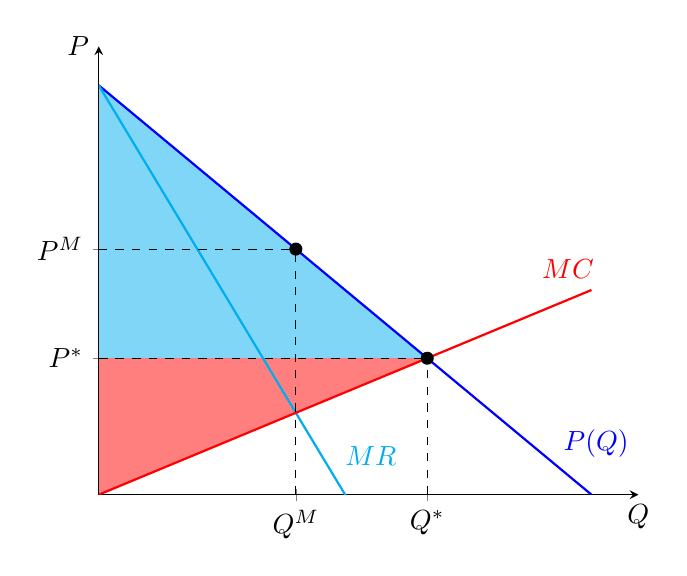
\begin{tikzpicture} 
\begin{axis}[
xlabel={$Q$}, 
ylabel={$P$},
axis lines= middle,
samples = 41, 
xmin = 0, xmax = 115,
ymin = 0, ymax = 115,
xtick = {0, 42, 70} ,
xticklabels={$0$, $Q^M$,  $Q^*$},
ytick = {35, 63},
yticklabels={$P^*$, $P^M$ },
legend pos = outer north east,
legend style={draw=none},   % If we don't want borders around the legend
xlabel style={below},
ylabel style={left}]

% Demand
\addplot[no marks, blue, thick, name path = demand, domain = 0:105] {105- 1*x};
% Marginal revenue
\addplot[no marks, cyan, thick, name path = MR, domain = 0:105] {105- 2*x};
% Marginal cost
\addplot[no marks, red, thick, name path = MC, red, domain = 0:105] {0.5*x };
% Monopoly Equilibrium price
\addplot[dashed, name path = pm, domain = 0:42] {63}; 
 % Competitive equilibrium price
\addplot[dashed, name path = pstar, domain = 0:70, black ] {35}; 
% Monopoly Equilibrium quantity
\addplot[dashed, black] coordinates {(42, 0) (42, 63)}; 
 % Competitive quantity
\addplot[dashed, black] coordinates {(70, 0) (70, 35)}; 
% Filling areas under the functions now
% Consumer surplus
\addplot [
thick,
color=cyan,
fill=cyan, 
fill opacity=0.5
]
fill between[
of= demand and pstar,
soft clip={domain=0:70},
];

% Producer surplus
\addplot [
thick,
color=red,
fill=red, 
fill opacity=0.5
]
fill between[
of= MC and pstar,
soft clip={domain=0:70},
];

\node[circle, scale = 0.5, fill = black] at (axis cs:70, 35) {};
\node[circle, scale = 0.5, fill = black] at (axis cs:42, 63) {};

% Label the curves
\node[blue] at (axis cs: 106, 13) {$P(Q)$};
\node[cyan] at (axis cs: 58, 10) {$MR$};
\node[red] at (axis cs: 100, 58) {$MC$};

\end{axis}

\end{tikzpicture}  % No space between the end of the first plot and the beginning of the second one if one wants them to be side by side
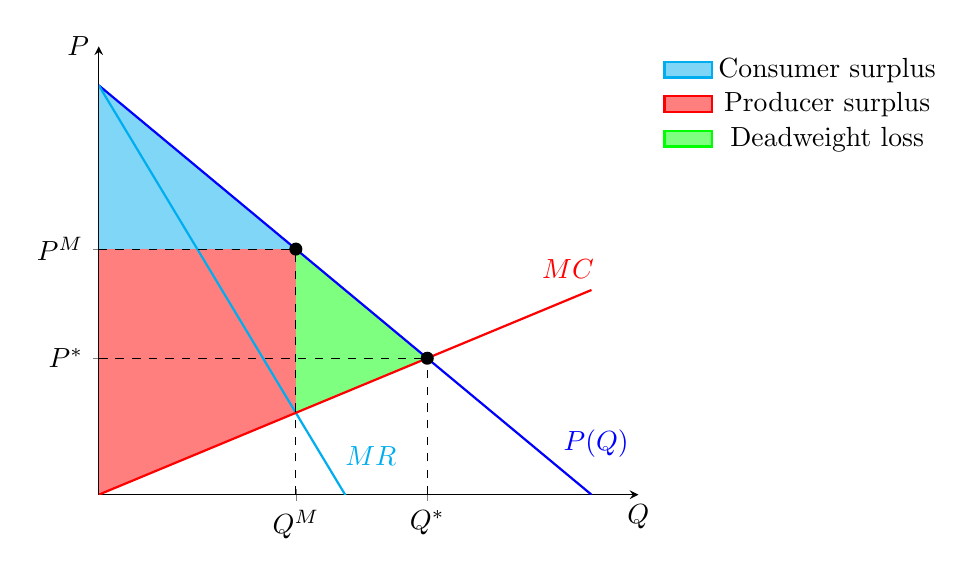
\begin{tikzpicture} 
\begin{axis}[
xlabel={$Q$}, 
ylabel={$P$},
axis lines= middle,
samples = 41, 
xmin = 0, xmax = 115,
ymin = 0, ymax = 115,
xtick = {0, 42, 70} ,
xticklabels={$0$, $Q^M$,  $Q^*$},
ytick = {35, 63},
yticklabels={$P^*$, $P^M$ },
legend pos = outer north east,
legend style={draw=none},   % If we don't want borders around the legend
xlabel style={below},
ylabel style={left}]

% Demand
\addplot[no marks, blue, thick, name path = demand, domain = 0:105] {105- 1*x};
% Marginal revenue
\addplot[no marks, cyan, thick, name path = MR, domain = 0:105] {105- 2*x};
% Marginal cost
\addplot[no marks, red, thick, name path = MC, red, domain = 0:105] {0.5*x };

\addplot[dashed, name path = pm, domain = 0:42] {63};   % Monopoly Equilibrium price
\addplot[dashed, name path = pstar, domain = 0:70, black ] {35};   % Competitive equilibrium price
\addplot[dashed, black] coordinates {(42, 0) (42, 63)};  % Monopoly Equilibrium quantity
\addplot[dashed, black] coordinates {(70, 0) (70, 35)};  % Competitive quantity
% Filling areas under the functions now
% Consumer surplus
\addplot [
thick,
color=cyan,
fill=cyan, 
fill opacity=0.5
]
fill between[
of= demand and pm,
soft clip={domain=0:42},
];

% Producer surplus
\addplot [
thick,
color=red,
fill=red, 
fill opacity=0.5
]
fill between[
of= MC and pm,
soft clip={domain=0:42},
];

% Deadweight loss
\addplot [
thick,
color= green,
fill=green, 
fill opacity=0.5
]
fill between[
of= demand and MC,
soft clip={domain=42:70},
];



\legend{,
	,
	,
	,
	,
	,
	,
	Consumer surplus,
	Producer surplus,
	Deadweight loss
}

\node[circle, scale = 0.5, fill = black] at (axis cs:70, 35) {};
\node[circle, scale = 0.5, fill = black] at (axis cs:42, 63) {};

% Label the curves
\node[blue] at (axis cs: 106, 13) {$P(Q)$};
\node[cyan] at (axis cs: 58, 10) {$MR$};
\node[red] at (axis cs: 100, 58) {$MC$};

\end{axis}

\end{tikzpicture}
\end{center}
\caption[Monopoly vs perfect competition outcomes]{Surpluses under perfect competition (left) and uniform monopoly pricing (right)}
\end{figure}

\subsection{Price discrimination: First degree}	


The following graphs show the monopoly outcome under uniform pricing versus first degree price discrimination. Under the latter, the monopolist is able to extract all the consumer surplus, leaving no blue area in the left graph.	
% Graph for surpluses with a profit maximizing monopoly VS first degree PD
% MC =  35
% MB = 105 - Q

% Monopoly equilibrium: (35, 70)
% Competitive equilibrium equilibrium: (70, 35)
\begin{figure}[H]
\begin{center}
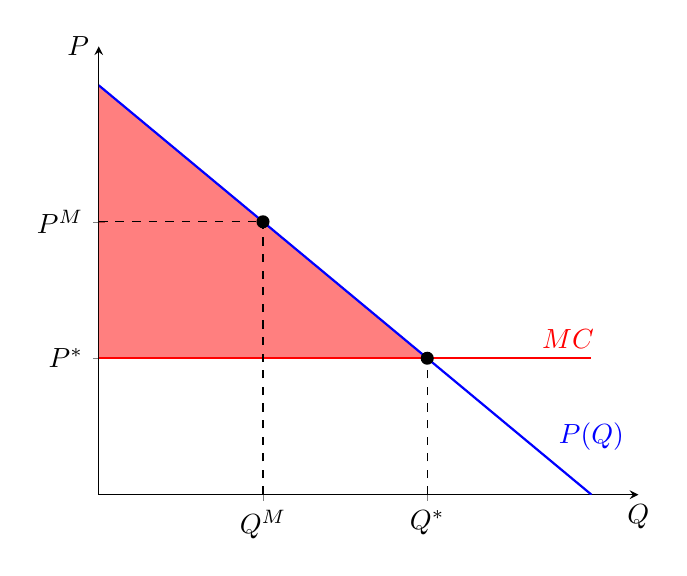
\begin{tikzpicture} 
\begin{axis}[
xlabel={$Q$}, 
ylabel={$P$},
axis lines= middle,
samples = 41, 
xmin = 0, xmax = 115,
ymin = 0, ymax = 115,
xtick = {0, 35, 70} ,
xticklabels={$0$, $Q^M$,  $Q^*$},
ytick = {35, 70},
yticklabels={$P^*$, $P^M$ },
legend pos = outer north east,
legend style={draw=none},   % If we don't want borders around the legend
xlabel style={below},
ylabel style={left}]

% Demand
\addplot[no marks, blue, thick, name path = demand, domain = 0:105] {105- 1*x};
% Marginal revenue
%\addplot[no marks, cyan, thick, name path = MR, domain = 0:105] {105- 2*x};
% Marginal cost
\addplot[no marks, red, thick, name path = MC, red, domain = 0:105] {35};
% Monopoly Equilibrium price
\addplot[dashed, name path = pm, domain = 0:35] {70};   
% Competitive equilibrium price
%\addplot[dashed, name path = pstar, domain = 0:70, black ] {35}; 
% Monopoly Equilibrium quantity
\addplot[dashed, black] coordinates {(35, 0) (35, 70)}; 
 % Competitive quantity
\addplot[dashed, black] coordinates {(70, 0) (70, 35)}; 

% Filling areas under the functions now
% Consumer surplus
%\addplot [
%thick,
%color=cyan,
%fill=cyan, 
%fill opacity=0.5
%]
%fill between[
%of= demand and MC,
%soft clip={domain=0:70},
%];

% Producer surplus (=consumer surplus in first degree PD)
\addplot [
thick,
color=red,
fill=red, 
fill opacity=0.5
]
fill between[
of= demand and MC,
soft clip={domain=0:70},
];

% Deadweight loss
%\addplot [
%thick,
%color= green,
%fill=green, 
%fill opacity=0.5
%]
%fill between[
%of= demand and MC,
%soft clip={domain=42:70},
%];



%\legend{,
%	,
%	,
%	,
%	,
%	Consumer surplus
%%	Producer surplus,
%%	Deadweight loss
%}

\node[circle, scale = 0.5, fill = black] at (axis cs:70, 35) {};
\node[circle, scale = 0.5, fill = black] at (axis cs:35, 70) {};

% Label the curves
\node[blue] at (axis cs: 105, 15) {$P(Q)$};
\node[red] at (axis cs: 100, 40) {$MC$};

\end{axis}

\end{tikzpicture}%
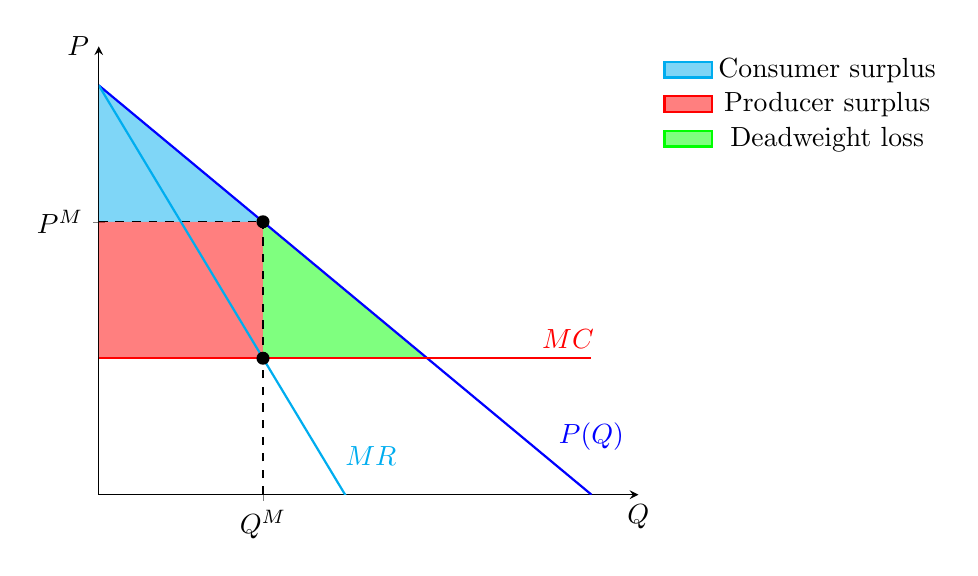
\begin{tikzpicture} 
	\begin{axis}[
xlabel={$Q$}, 
ylabel={$P$},
axis lines= middle,
samples = 41, 
xmin = 0, xmax = 115,
ymin = 0, ymax = 115,
xtick = {0, 35} ,
xticklabels={$0$, $Q^M$},
ytick = {70},
yticklabels={ $P^M$ },
legend pos = outer north east,
legend style={draw=none},   % If we don't want borders around the legend
xlabel style={below},
ylabel style={left}]
		
% Demand
\addplot[no marks, blue, thick, name path = demand, domain = 0:105] {105- 1*x};
% Marginal revenue
\addplot[no marks, cyan, thick, name path = MR, domain = 0:105] {105- 2*x};
% Marginal cost
\addplot[no marks, red, thick, name path = MC, red, domain = 0:105] {35};
% Monopoly Equilibrium price
\addplot[dashed, name path = pm, domain = 0:35] {70}; 
% Competitive equilibrium price
%\addplot[dashed, name path = pstar, domain = 0:70, black ] {35};
% Monopoly Equilibrium quantity
\addplot[dashed, black] coordinates {(35, 0) (35, 70)};  

% Filling areas under the functions now
% Consumer surplus
\addplot [
thick,
color=cyan,
fill=cyan, 
fill opacity=0.5
]
fill between[
of= demand and pm,
soft clip={domain=0:35},
];
		
% Producer surplus
\addplot [
thick,
color=red,
fill=red, 
fill opacity=0.5
]
fill between[
of= MC and pm,
soft clip={domain=0:35},
];
		
% Deadweight loss
\addplot [
thick,
color= green,
fill=green, 
fill opacity=0.5
]
fill between[
of= demand and MC,
soft clip={domain=35:70},
];
		
\legend{,
	,
	,
	,
	,
	Consumer surplus,
	Producer surplus,
	Deadweight loss
}
		
\node[circle, scale = 0.5, fill = black] at (axis cs:35, 35) {};
\node[circle, scale = 0.5, fill = black] at (axis cs:35, 70) {};
		
% Label the curves
\node[blue] at (axis cs: 105, 15) {$P(Q)$};
\node[cyan] at (axis cs: 58, 10) {$MR$};
\node[red] at (axis cs: 100, 40) {$MC$};
	
\end{axis}
	
\end{tikzpicture}
\end{center}
\caption[Uniform pricing vs $1^{st}$ degree price discrimination]{Monopoly outcome under first degree price discrimination (left) vs uniform pricing (right). }
\end{figure}
	
\section{Externalities} \label{externalities}
This section displays the different impacts of positive/negative externalities in the case of production/consumption. Note the use of \texttt{fill between}	to display the different surpluses and deadweight losses.

% Graph for surpluses with a negative consumption externality.
% SMC = 0.5Q
% PMB = 60 - 0.5Q
% SED = 20
% SMB = 40 - 0.5Q
% Market equilibrium: (60, 30)
% Socially efficient level: (40, 20)
\begin{figure}[H]
\begin{center}
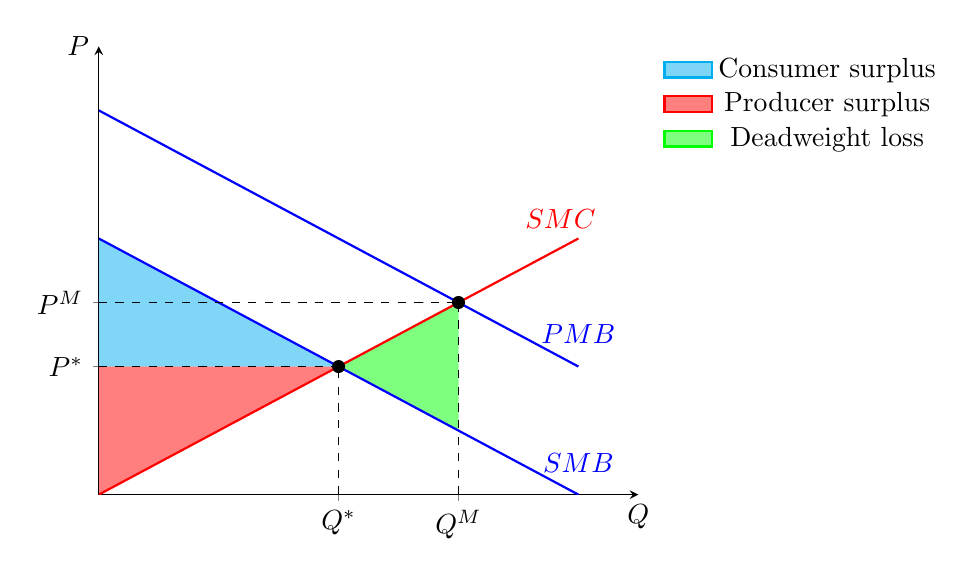
\begin{tikzpicture} 
\begin{axis}[
xlabel={$Q$}, 
ylabel={$P$},
axis lines= middle,
samples = 41, 
xmin = 0, xmax = 90,
ymin = 0, ymax = 70,
xtick = {0, 40, 60} ,
xticklabels={$0$, $Q^*$, $Q^M$},
ytick = {20, 30},
yticklabels={$P^*$, $P^M$  },
legend pos = outer north east,
legend style={draw=none},   % If we don't want borders around the legend
xlabel style={below},
ylabel style={left}]

% Social marginal benefit
\addplot[ thick, name path = SMB, blue, domain = 0:80] {40- 0.5*x};
% Private marginal benefit
\addplot[thick, name path = PMB, blue, domain = 0:80] {40 + 20 - 0.5*x};
% Social marginal cost
\addplot[thick, name path = SMC, red, domain = 0:80] {0.5*x};
 % Market Equilibrium price
\addplot[dashed, name path = pm, domain = 0:60] {30}; 
 % Socially efficient price
\addplot[dashed, name path = pstar, domain = 0:40, black ] {20};  
 % Market Equilibrium quantity
\addplot[dashed, black] coordinates {(60, 0) (60, 30)}; 
% Socially efficient quantity
\addplot[dashed, black] coordinates {(40, 0) (40, 20)};  
% Filling areas under the functions now
% Consumer surplus
\addplot [
thick,
color=cyan,
fill=cyan, 
fill opacity=0.5
]
fill between[
of=SMB and pstar,
soft clip={domain=0:60},
];

% Producer surplus
\addplot [
thick,
color=red,
fill=red, 
fill opacity=0.5
]
fill between[
of=pstar and SMC,
soft clip={domain=0:60},
];

% Deadweight loss
\addplot [
thick,
color=green,
fill=green, 
fill opacity=0.5
]
fill between[
of=SMC and SMB,
soft clip={domain=40:60},
];
% The legend lists all the curves created before. So many entries are empty as not needed to appear in the legend
\legend{,
	,
	,
	,
	,
	,
	,
	Consumer surplus,
	Producer surplus,
	Deadweight loss
}

\node[circle, scale = 0.5, fill = black] at (axis cs:60, 30) {};
\node[circle, scale = 0.5, fill = black] at (axis cs:40, 20) {};

% Label the SMB, PMC and SMC curves
\node[blue] at (axis cs: 80, 5) {$SMB$};
\node[blue] at (axis cs: 80, 25) {$PMB$};
\node[red] at (axis cs: 77, 43) {$SMC$};

\end{axis}

\end{tikzpicture}
\end{center}
\caption[Negative consumption externality]{Negative consumption externality}
\end{figure}

	
% Graph for surpluses with a negative production externality.
% MC = 0.5Q
% MB = 105 - Q
% SEC = 30
% Market equilibrium: (70, 35)
% Socially efficient level: (50, 55)
\begin{figure}[H]
\begin{center}
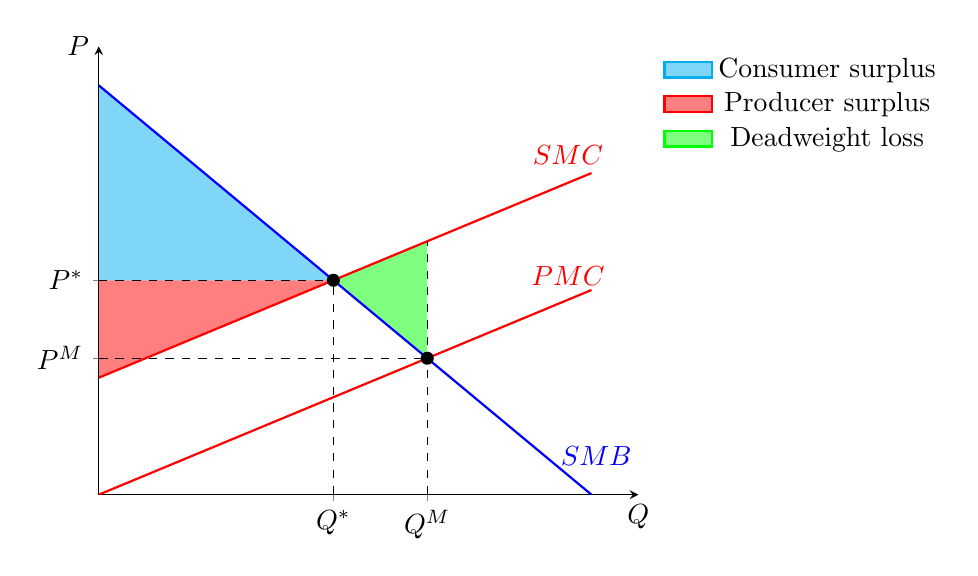
\begin{tikzpicture} 
\begin{axis}[
xlabel={$Q$}, 
ylabel={$P$},
axis lines= middle,
samples = 41, 
xmin = 0, xmax = 115,
ymin = 0, ymax = 115,
xtick = {0, 50, 70} ,
xticklabels={$0$, $Q^*$, $Q^M$},
ytick = {35, 55},
yticklabels={$P^M$, $P^*$ },
legend pos = outer north east,
legend style={draw=none},   % If we don't want borders around the legend
xlabel style={below},
ylabel style={left}]

% Social marginal benefit
\addplot[ thick, blue, name path = SMB, domain = 0:105] {105- 1*x};
% Private marginal cost
\addplot[ thick, red, name path = PMC, domain = 0:105] {0.5*x};
% Social marginal cost
\addplot[ thick, red, name path = SMC, domain = 0:105] {0.5*x + 30};
% Market Equilibrium price
\addplot[dashed, name path = pm, domain = 0:70] {35};  
 % Socially efficient price
\addplot[dashed, name path = pstar, domain = 0:50, black ] {55}; 
% Market Equilibrium quantity
\addplot[dashed, black] coordinates {(70, 0) (70, 65)};  
% Socially efficient quantity
\addplot[dashed, black] coordinates {(50, 0) (50, 55)};  
% Filling areas under the functions now
% Consumer surplus
\addplot [
thick,
color=cyan,
fill=cyan, 
fill opacity=0.5
]
fill between[
of=SMB and pstar,
soft clip={domain=0:50},
];

% Producer surplus
\addplot [
thick,
color=red,
fill=red, 
fill opacity=0.5
]
fill between[
of=pstar and SMC,
soft clip={domain=0:50},
];

% Deadweight loss
\addplot [
thick,
color=green,
fill=green, 
fill opacity=0.5
]
fill between[
of=SMC and SMB,
soft clip={domain=50:70},
];

\legend{,
	,
	,
	,
	,
	,
	,
	Consumer surplus,
	Producer surplus,
	Deadweight loss
}

\node[circle, scale = 0.5, fill = black] at (axis cs:70, 35) {};
\node[circle, scale = 0.5, fill = black] at (axis cs:50, 55) {};

% Label the SMB, PMC and SMC
\node[blue] at (axis cs: 106, 10) {$SMB$};
\node[red] at (axis cs: 100, 56) {$PMC$};
\node[red] at (axis cs: 100, 87) {$SMC$};

\end{axis}

\end{tikzpicture}	
\end{center}
\caption[Negative production externality]{Negative production externality}
\end{figure}

This last graph shows the design of a \textbf{Pigouvian tax} in the case where there is a negative production externality. Note that the marginal external cost is not constant here.
% Graph for a Pigouvian tax in the case of a negative production externality.
% MC = 0.5Q
% MB = 105 - Q
% MEC = 0.5Q   Marginal external cost
% Market equilibrium: (70, 35)
% Socially efficient level: (50, 55)
\begin{figure}[H]
\begin{center}
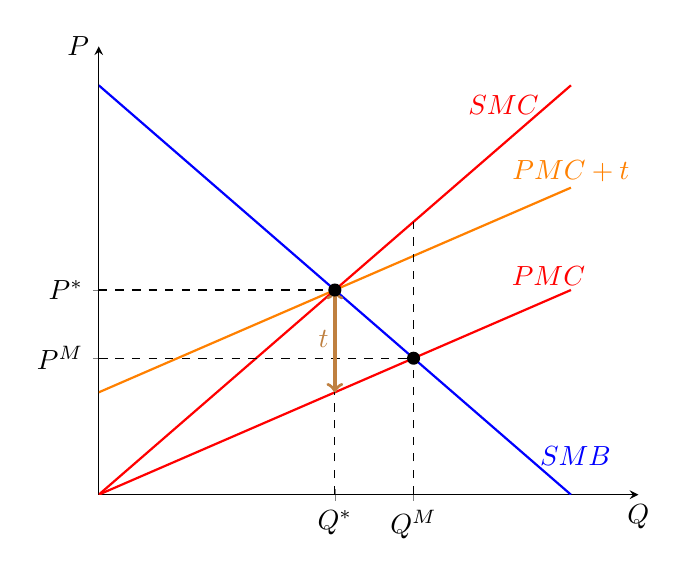
\begin{tikzpicture} 
\begin{axis}[
xlabel={$Q$}, 
ylabel={$P$},
axis lines= middle,
samples = 41, 
xmin = 0, xmax = 120,
ymin = 0, ymax = 115,
xtick = {0, 52.5, 70} ,
xticklabels={$0$, $Q^*$, $Q^M$},
ytick = {35, 52.5},
yticklabels={$P^M$, $P^*$ },
legend pos = outer north east,
legend style={draw=none},   % If we don't want borders around the legend
xlabel style={below},
ylabel style={left}]

% Social marginal benefit
\addplot[no marks, thick, blue, name path = SMB, domain = 0:105] {105- 1*x};
% Private marginal cost
\addplot[no marks, thick, name path = PMC, red, domain = 0:105] {0.5*x};
% Private marginal cost + Pigouvian tax of 52.5/2 = 26.25
\addplot[no marks, thick, name path = PMC, orange, domain = 0:105] {0.5*x + 26.25};
% Social marginal cost
\addplot+[no marks, thick, name path = SMC, red, domain = 0:105] {1*x };
% Market Equilibrium price
\addplot[dashed, name path = pm, domain = 0:70] {35};   
% Socially efficient price
\addplot[ dashed, name path = pstar, domain = 0:52.5, black ] {52.5};   
 % Market Equilibrium quantity
\addplot[dashed, black] coordinates {(70, 0) (70, 70)};
 % Socially efficient quantity
\addplot[ dashed, black] coordinates {(52.5, 0) (52.5, 52.5)}; 
  
% The Pigouvian tax
%\addplot[no marks, thick, orange] coordinates {(52.5, 26.25) (52.5, 52.5)};   % does not make arrows...
\draw [brown, very thick] [<->](52.5, 26.25)--(52.5, 52.5) ;

% Filling areas under the functions now
% Consumer surplus
%\addplot [
%thick,
%color=cyan,
%fill=cyan, 
%fill opacity=0.5
%]
%fill between[
%of=SMB and pstar,
%soft clip={domain=0:52.5},
%];

% Producer surplus
%\addplot [
%thick,
%color=red,
%fill=red, 
%fill opacity=0.5
%]
%fill between[
%of=pstar and SMC,
%soft clip={domain=0:52.5},
%];

% Deadweight loss
%\addplot [
%thick,
%color=green,
%fill=green, 
%fill opacity=0.5
%]
%fill between[
%of=SMC and SMB,
%soft clip={domain=52.5:70},
%];

%\legend{,
%	,
%	,
%	,
%	,
%	,
%	,
%	Consumer surplus,
%	Producer surplus,
%	Deadweight loss
%}

\node[circle, scale = 0.5, fill = black] at (axis cs:70, 35) {};
\node[circle, scale = 0.5, fill = black] at (axis cs:52.5, 52.5) {};

% Label the SMB, PMC, SMC and the Pigouvian tax
\node[blue] at (axis cs: 106, 10) {$SMB$};
\node[red] at (axis cs: 100, 56) {$PMC$};
\node[orange] at (axis cs: 105, 83) {$PMC + t$};
\node[red] at (axis cs: 90, 100) {$SMC$};
\node[brown] at (axis cs: 50, 40) {$t$};

\end{axis}

\end{tikzpicture}
\end{center}
\caption[Pigouvian tax]{Pigouvian tax for a negative production externality}
\end{figure}
	
\section{Taxation}
This section show various graphs among which are found:
\begin{itemize}
\item The Lorenz curve
\item The impact of a tax/subsidy on consumer surplus, producer surplus, government revenue/cost and the resulting deadweight loss.
\item Tax incidence, shown through graphs displaying a more inelastic demand than supply
\end{itemize}
	
% Reset the graph sizes	
\pgfplotsset{   % We can resize the plots with this command
	normalsize,
	%legend style={legend pos=north east}
	legend style={
		at={(0.01,0.01)},
		anchor=south west,
	},
}%		
	
% Lorenz curve
\begin{figure}[H]
\begin{center}
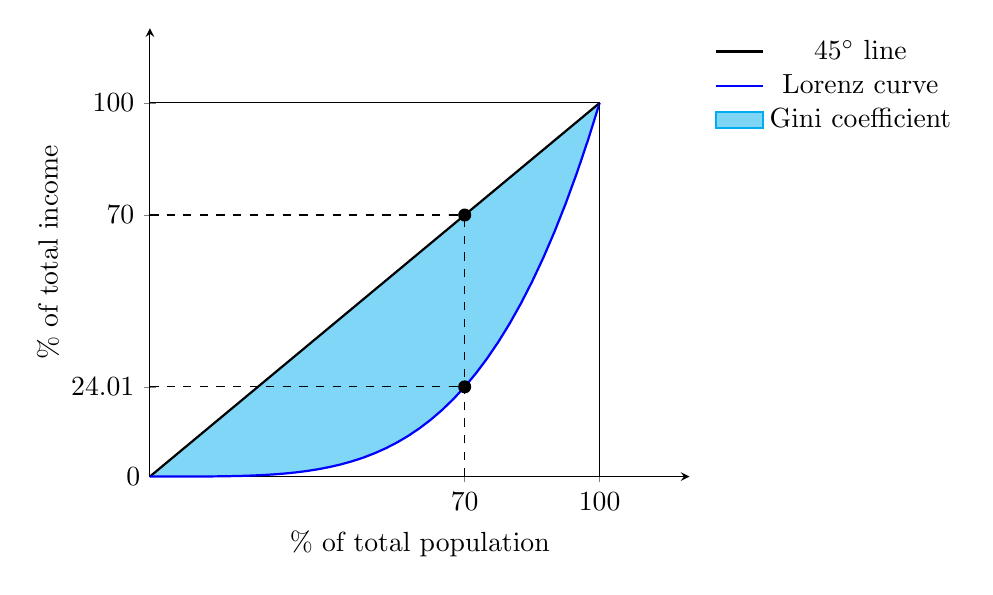
\begin{tikzpicture} 
\begin{axis}[
xlabel={$\%$ of total population}, 
ylabel={$\%$ of total income},
axis lines= middle,
samples = 41, 
clip=false,
xmin = 0, xmax = 1.2,
ymin = 0, ymax = 1.2,
xtick = {0, 0.7, 1},
ytick = { 0.2401, 0.7, 1},
xticklabels = {$0$, $70$, $100$},
yticklabels = { $24.01$, $70$, $100$},
legend pos = outer north east,
legend style={draw=none},   % If we don't want borders around the legend
x label style={at={(axis description cs:0.5,-0.1)},anchor=north},
y label style={at={(axis description cs:-0.15, 0.5)},rotate=90,anchor=south}
%xlabel style={below},
%ylabel style={left}
]
% The 45 degrees line
\addplot[black, thick, no marks, name path = equality, domain = 0:1] {x};
% Lorenz curve
\addplot[blue, thick, no marks, name path = lorenz, domain = 0:1] {x^4};

% Showing the Gini coefficient
% Gini
\addplot [
thick,
color=cyan,
fill=cyan, 
fill opacity=0.5
]
fill between[
of=equality and lorenz,
soft clip={domain=0:1},
];
 
\legend{$45^{\circ}$ line,
	Lorenz curve,
	Gini coefficient
}

% Pick a random point on the 45 degrees line to illustrate
\node[circle, scale = 0.5, fill = black] at (axis cs:0.7, 0.7) {};   
\addplot[ dashed, domain = 0:0.7] {0.7};   
\addplot[ dashed, black] coordinates {(0.7, 0) (0.7, 0.7)};

% Pick a random point on the Lorenz curve to illustrate
\node[circle, scale = 0.5, fill = black] at (axis cs:0.7, 0.2401) {};   
\addplot[ dashed, domain = 0:0.7] {0.2401};   
\addplot[ dashed, black] coordinates {(0.7, 0) (0.7, 0.2401)};

%\node[circle, scale = 0.5, fill = black] at (axis cs:1, 1) {};   
\addplot[ domain = 0:1] {1};   
\addplot[ black] coordinates {(1, 0) (1,1)};

% Node of the origin (xticklabel can't do it for some reason)
\node at (axis cs:0, 0) [black, anchor=east] {$0$};

\end{axis}

\end{tikzpicture}
\caption[Lorenz curve]{Lorenz curve and Gini coefficient}
\end{center}
\end{figure}


% 1st plot: effect of a quantity tax of 20 on consumers. The graph shows before tax
% Demand: P = 80 - 2Q
% Supply: P = 2Q
% Equilibrium = (20, 40)
\begin{figure}[H]
\begin{center}

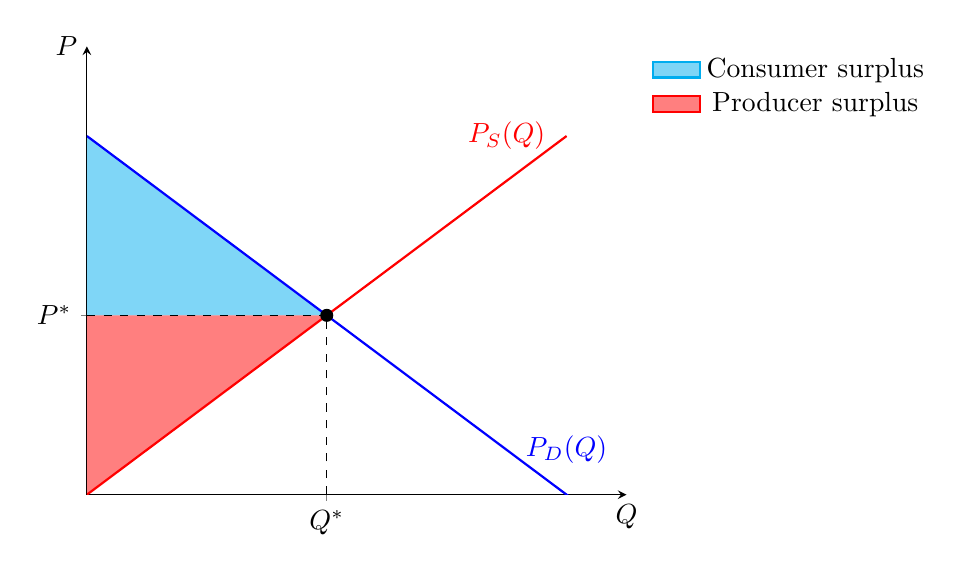
\begin{tikzpicture} 
\begin{axis}[
xlabel={$Q$}, 
ylabel={$P$},
axis lines= middle,
samples = 41, 
xmin = 0, xmax = 45,
ymin = 0, ymax = 100,
xtick = {0, 20},
ytick = 40,
xticklabels = {$0$, $Q^*$},
yticklabels = {$P^*$},
legend pos = outer north east,
legend style={draw=none},   % If we don't want borders around the legend
xlabel style={below},
ylabel style={left}]
% Demand
\addplot[thick, blue, name path = demand, domain = 0:45] {80- 2*x};
% Supply
\addplot[thick, red, name path = supply, domain = 0:40] {2*x};
% Equilibrium price
\addplot[dashed, name path = pstar, domain = 0:20] {40}; 
% Equilibrium quantity
\addplot[dashed, black] coordinates {(20, 0) (20, 40)};  
% Filling areas under the functions now
% Consumer surplus
\addplot [
thick,
color=cyan,
fill=cyan, 
fill opacity=0.5
]
fill between[
of=demand and pstar,
soft clip={domain=0:20},
];

% Producer surplus
\addplot [
thick,
color=red,
fill=red, 
fill opacity=0.5
]
fill between[
of = pstar and supply,
soft clip={domain=0:20},
];

\legend{,
       ,
       ,
       ,
       Consumer surplus,
       Producer surplus,
}

% Label the demand and supply
\node[blue] at (axis cs: 40, 10) {$P_D(Q)$};
\node[red] at (axis cs: 35, 80) {$P_S(Q)$};
\node[circle, scale = 0.5, fill = black] at (axis cs: 20, 40) {};   

% Label the CS and PS
%\node[blue] at (axis cs: 8, 50) {$CS$};
%\node[red] at (axis cs: 8, 30) {$PS$};

%\node[circle, scale = 0.5, fill = black, pin=90:{$(Q^*, P^*)$}] at (axis cs:20, 40) {};   % shows the equilibrium price and quantity on the graph

\end{axis}

\end{tikzpicture}
\caption[Surpluses under perfect competition]{Surpluses under perfect competition}
\end{center}
\end{figure}

% 2nd plot for consumer surplus with a quantity tax of 20
\begin{figure}[H]
\begin{center}
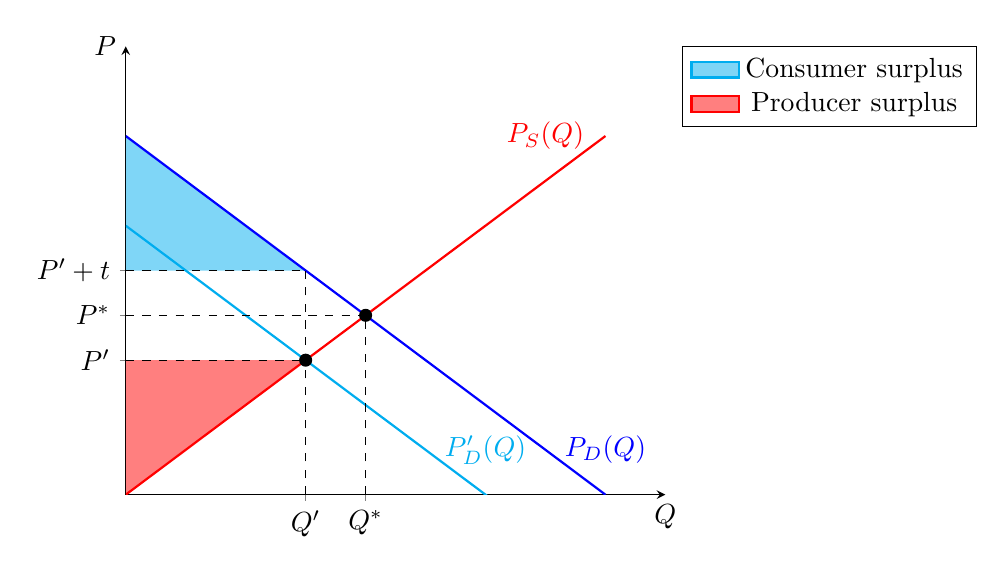
\begin{tikzpicture} 
\begin{axis}[
xlabel={$Q$}, 
ylabel={$P$},
axis lines= middle,
samples = 41, 
xmin = 0, xmax = 45,
ymin = 0, ymax = 100,
xtick = {0, 15, 20},
ytick = {30, 40, 50},
xticklabels = {$0$, $Q^\prime$, $Q^*$},
yticklabels = {$P^\prime$, $P^*$, $P^\prime + t$},
legend pos = outer north east,
xlabel style={below},
ylabel style={left}]
% Inverse Demand
\addplot[ thick, blue, name path = demand, domain = 0:40] {80- 2*x};
% New Inverse Demand
\addplot[ thick, name path = new demand, cyan, domain = 0:40] {80 - 20 - 2*x};
% Inverse Supply
\addplot[thick, name path = supply, red, domain = 0:40] {2*x};
% Old Equilibrium price
\addplot[dashed, name path = pstar, domain = 0:20] {40};  
 % New Equilibrium price
\addplot[dashed, name path = pprime, domain = 0:15 ] {30}; 
% New price + t
\addplot[dashed, name path = pprime-with-t, domain = 0:15] {50}; 
% Old Equilibrium quantity
\addplot[dashed, black] coordinates {(20, 0) (20, 40)};  
\addplot[dashed, black] coordinates {(15, 0) (15, 50)}; 

% Filling areas under the functions now
% Consumer surplus
\addplot [
thick,
color=cyan,
fill=cyan, 
fill opacity=0.5
]
fill between[
of=demand and pprime-with-t,
soft clip={domain=0:15},
];

% Producer surplus
\addplot [
thick,
color=red,
fill=red, 
fill opacity=0.5
]
fill between[
of=pprime and supply,
soft clip={domain=0:20},
];

\legend{,
        ,
	    ,
	    ,
	    ,
	    ,
	    ,
	    ,
     	Consumer surplus,
	    Producer surplus
}

\node[circle, scale = 0.5, fill = black] at (axis cs:20, 40) {};
\node[circle, scale = 0.5, fill = black] at (axis cs:15, 30) {};

% Label the demands and supply
\node[blue] at (axis cs: 40, 10) {$P_D(Q)$};
\node[red] at (axis cs: 35, 80) {$P_S(Q)$};
\node[cyan] at (axis cs: 30, 10) {$P^\prime_D(Q)$};

\end{axis}

\end{tikzpicture}
\end{center}
\caption[Quantity tax on demand]{Effect of a quantity tax on demand}
\end{figure}

% 3rd plot for surpluses with a quantity tax of 20. Same graph as the previous one, but includes the government revenue and the DWL
\begin{figure}[H]
\begin{center}
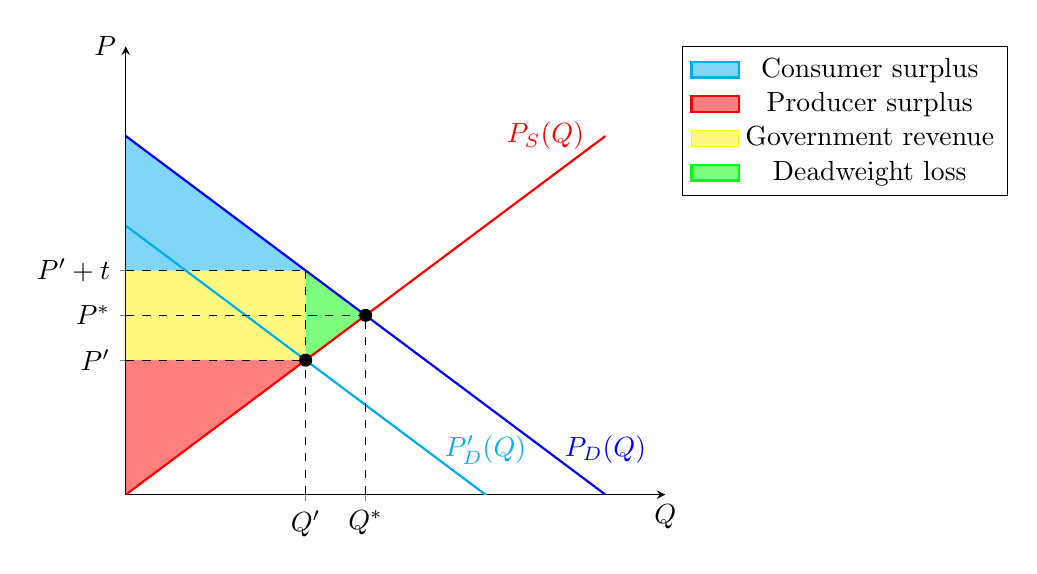
\begin{tikzpicture} 
\begin{axis}[
xlabel={$Q$}, 
ylabel={$P$},
axis lines= middle,
samples = 41, 
xmin = 0, xmax = 45,
ymin = 0, ymax = 100,
xtick = {0, 15, 20} ,
xticklabels={$0$, $Q^\prime$, $Q^*$},
ytick = {30, 40, 50},
yticklabels={$P^\prime$, $P^*$, $P^\prime+t$ },
legend pos = outer north east,
xlabel style={below},
ylabel style={left}]
% Inverse Demand
\addplot+[no marks, thick, name path = demand, domain = 0:40] {80- 2*x};
% New Inverse Demand
\addplot+[no marks, thick, name path = new demand, cyan, domain = 0:40] {80 - 20 - 2*x};
% Inverse Supply
\addplot+[no marks, thick, name path = supply, red, domain = 0:40] {2*x};
\addplot[dashed, name path = pstar, domain = 0:20] {40};   % Old Equilibrium price
\addplot[dashed, name path = pprime, domain = 0:15, black ] {30};   % New Equilibrium price
\addplot[ dashed, name path = pprime-with-t, domain = 0:15, black] {50}; % New price + t 
\addplot[dashed, black] coordinates {(20, 0) (20, 40)};  % Old Equilibrium quantity
\addplot[dashed, black] coordinates {(15, 0) (15, 50)};  % New Equilibrium quantity
%\addplot[thick, no marks, brown] coordinates {(15, 30) (15, 50)};  % New Equilibrium quantity
% Filling areas under the functions now
% Consumer surplus
\addplot [
thick,
color=cyan,
fill=cyan, 
fill opacity=0.5
]
fill between[
of=demand and pprime-with-t,
soft clip={domain=0:15},
];

% Producer surplus
\addplot [
thick,
color=red,
fill=red, 
fill opacity=0.5
]
fill between[
of=pprime and supply,
soft clip={domain=0:20},
];

% Government revenue
\addplot[
%pattern = flexible hatch,
yellow,
fill=yellow, 
fill opacity=0.5,
%postaction={pattern = north east lines, opacity = .5}
]
fill between[
of=pprime-with-t and pprime,
soft clip={domain=0:15},
%every segment no 1/.style={pattern = north west lines},
];


% Deadweight loss
\addplot [
thick,
color=green,
fill=green, 
fill opacity=0.5
]
fill between[
of=demand and supply,
soft clip={domain=15:20},
];

\legend{,
	,
	,
	,
	,
	,
	,
	,
	Consumer surplus,
	Producer surplus,
	Government revenue,
	Deadweight loss
}

\node[circle, scale = 0.5, fill = black] at (axis cs:20, 40) {};
\node[circle, scale = 0.5, fill = black] at (axis cs:15, 30) {};
% Label the demands and supply
\node[blue] at (axis cs: 40, 10) {$P_D(Q)$};
\node[red] at (axis cs: 35, 80) {$P_S(Q)$};
\node[cyan] at (axis cs: 30, 10) {$P^\prime_D(Q)$};

\end{axis}
\end{tikzpicture}
\end{center}
\caption[Surpluses under quantity tax]{Surpluses and deadweight loss under a quantity tax on consumers}
\end{figure}

% 5th plot for surpluses with a quantity tax of 35 and a very inelastic demand
% Demand is P(Q) = 140 - 5Q
% Supply = 2Q
% Original equilibrium = (20, 40)
% New equilibrium = (15, 30)
\begin{figure}[H]
\begin{center}
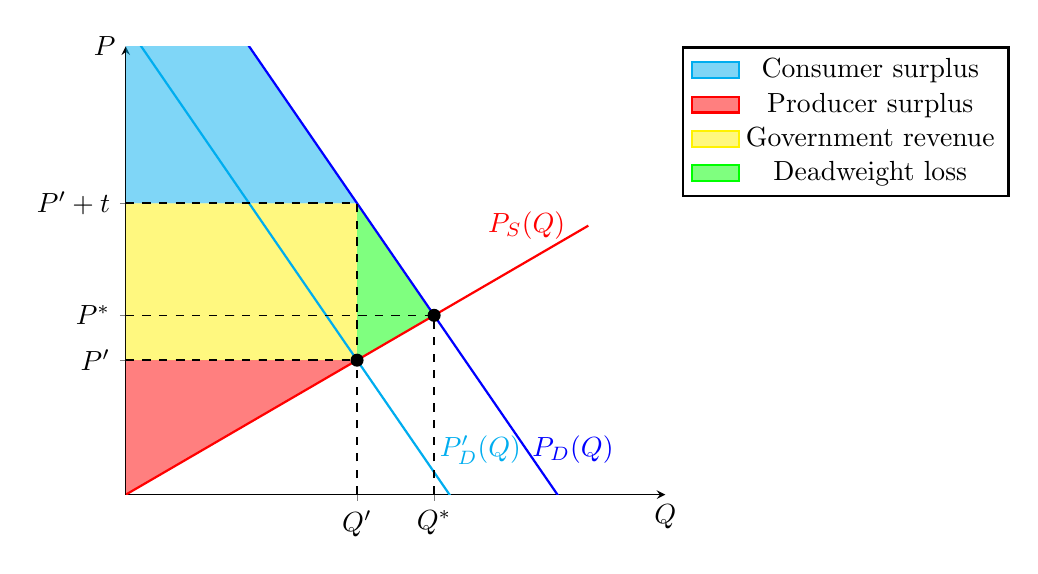
\begin{tikzpicture} 
\begin{axis}[
xlabel={$Q$}, 
ylabel={$P$},
axis lines= middle,
samples = 41, 
xmin = 0, xmax = 35,
ymin = 0, ymax = 100,
xtick = {0, 15, 20} ,
xticklabels={$0$, $Q^\prime$, $Q^*$},
ytick = {30, 40, 65},
yticklabels={$P^\prime$, $P^*$, $P^\prime+t$ },
% grid, 
thick,       
domain = 0:40,
legend pos = outer north east,
xlabel style={below},
ylabel style={left}   ]
% Inverse Demand
\addplot+[thick, no marks, name path = demand, domain = 0:30] {140- 5*x};
% New Inverse Demand
\addplot+[thick, no marks, name path = new demand, cyan, domain = 0:30] {140 - 35 - 5*x};
% Inverse Supply
\addplot+[thick, no marks, name path = supply, red, domain = 0:30] {2*x};
\addplot[dashed, name path = pstar, domain = 0:20] {40};   % Old Equilibrium price
\addplot[thick, dashed, name path = pprime, domain = 0:15, black ] {30};   % New Equilibrium price
\addplot[thick, dashed, name path = pprime-with-t, domain = 0:15, black] {65};   
\addplot[thick, dashed, black] coordinates {(20, 0) (20, 40)};  % Old Equilibrium quantity
\addplot[thick, dashed, black] coordinates {(15, 0) (15, 65)};  % New Equilibrium quantity
%\addplot[thick, no marks, brown] coordinates {(15, 30) (15, 65)};  % New Equilibrium quantity
% Filling areas under the functions now
% Consumer surplus
\addplot [
thick,
color=cyan,
fill=cyan, 
fill opacity=0.5
]
fill between[
of=demand and pprime-with-t,
soft clip={domain=0:15},
];

% Producer surplus
\addplot [
thick,
color=red,
fill=red, 
fill opacity=0.5
]
fill between[
of=pprime and supply,
soft clip={domain=0:15},
];

% Government revenue
\addplot[
%pattern = flexible hatch,
yellow,
fill=yellow, 
fill opacity=0.5,
%postaction={pattern = north east lines, opacity = .5}
]
fill between[
of=pprime-with-t and pprime,
soft clip={domain=0:15},
%every segment no 1/.style={pattern = north west lines},
];


% Deadweight loss
\addplot [
thick,
color=green,
fill=green, 
fill opacity=0.5
]
fill between[
of=demand and supply,
soft clip={domain=15:20},
];

\legend{,
	,
	,
	,
	,
	,
	,
	,
	Consumer surplus,
	Producer surplus,
	Government revenue,
	Deadweight loss
}

\node[circle, scale = 0.5, fill = black] at (axis cs:20, 40) {};
\node[circle, scale = 0.5, fill = black] at (axis cs:15, 30) {};

% Label the demands and supply
\node[blue] at (axis cs: 29, 10) {$P_D(Q)$};
\node[red] at (axis cs: 26, 60) {$P_S(Q)$};
\node[cyan] at (axis cs: 23, 10) {$P^\prime_D(Q)$};

\end{axis}

\end{tikzpicture}
\end{center}
\caption[Quantity tax on an inelastic demand]{Surpluses and deadweight loss under a quantity tax on an inelastic demand}
\end{figure}
	
\section{Labour Economics}
This section shows labor supply decisions in a leisure/consumption graph. A Cobb-Douglas utility function is used. Note that in the graph below, \texttt{legend}	is not declared , rather \texttt{addlegendentry} is used immediately after declaring the function. It is another way to declare the legend, although I prefer to dedicate a whole environment to it using \texttt{legend}.

% Labor decision plot, with w = p = 1, Income = 8, T = 16. The utility function is u = (CL)^(1/2) and the optimal bundle is located at (12, 12). 
\begin{figure}[H]
\begin{center}
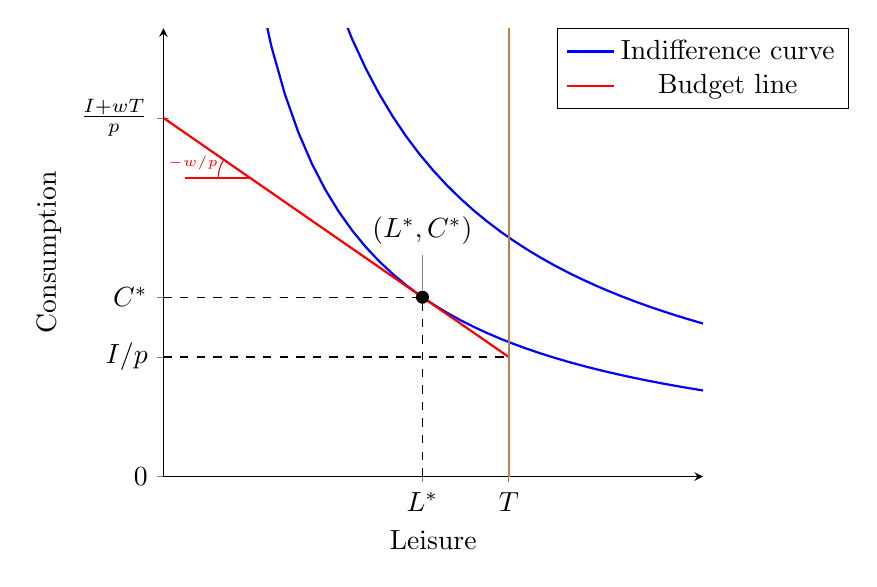
\begin{tikzpicture} 
\begin{axis}[          
xlabel={Leisure}, 
ylabel={Consumption},
axis lines=left,
samples = 41,   % Play with this number to see how more or less choppy the graphed functions look like
domain = 0:25,
ymin = 0,
ymax = 30,
%legend pos =  north east,
legend style={ at={(1, 1)} , anchor = north},  % The coordinates are in terms of the graph box. They are between 0 and 1. Add "draw=none" if one does not want borders around the legend
xtick = {12, 16},
xticklabels = { $L^*$, $T$},
ytick = {0, 8, 12, 24},
yticklabels = {$0$, $I/p$, $C^*$, $\frac{I+wT}{p}$}
]
% First indifference curve, on which the optimal bundle will be located:
\addplot[thick, blue, name path = Indifference] { 12^2/x };   
%\addplot+[mark = none, name path global = Indifference] { 12^2/x };
\addlegendentry{Indifference curve}
% Budget line
\addplot[thick, red, name path = Budget, domain = 0:16] {24 - x};   
%\addplot+[mark = none, name path global = Budget, domain = 0:16] {24 - x};   
\addlegendentry{Budget line}   %...

% Another indifference curve
\addplot[thick, blue] { 16^2/x };   
%\addplot+[mark = none, blue] { 16^2/x };

% Vertical bar for the maximum amount of time
\addplot[thick, brown] coordinates {(16, 0) (16, 30)};  
% Consumption if leisure equals T: I/p 
\addplot[dashed, domain = 0:16 , black] {8};   
 % Optimal leisure decision
\addplot[dashed, black, thin] coordinates {(12, 0) (12, 12)};  
% Optimal consumption decision
\addplot[dashed, domain = 0:12 , black, thin] {12};  
% Location of the optimal bundle
\node[circle, scale = 0.5, fill = black, pin=90:{$(L^*, C^*)$}] at (axis cs:12, 12) {};
% For the angle of the budget line
\addplot[no marks, domain = 1:4, red, thick] {20};
%\node[circle, scale = 0.5, fill = black, pin=90:{$(L^*, C^*)$}] at (axis cs:12, 12) {};
\coordinate (A) at (3, 21);
\coordinate (B) at (4, 20);
\coordinate (C) at (3, 20);
\pic [draw=red, -, angle radius=.4cm]{angle = A--B--C};
\node at (axis cs:3,21) [red, anchor=east, thick] {\tiny $-w/p$};
%\draw
%(3, 21) coordinate (A)
%-- (4, 20)coordinate (B)
%-- (3, 20)coordinate (C)

%\tikzMarkAngle{(A)}{(B)}{(C)}
\end{axis}


\end{tikzpicture}
\end{center}
\caption[Optimal labor-leisure decision]{Optimal consumption-leisure decision}
\end{figure}	
	
The graph below shows the impact of a wage tax on labor supply (in the example shown here, the new optimal labor supply is lower as the \textbf{substitution effect} dominates the \textbf{income effect}).	
	
% Labor decision plot with a wage tax t = 0.5, with w = p = 1, Income = 4, T = 20. The utility function is u = (CL)^(1/2) and the old optimal bundle is located at (12, 12). The new optimal bundle is located at (14, 7) 
\begin{figure}[H]
\begin{center}
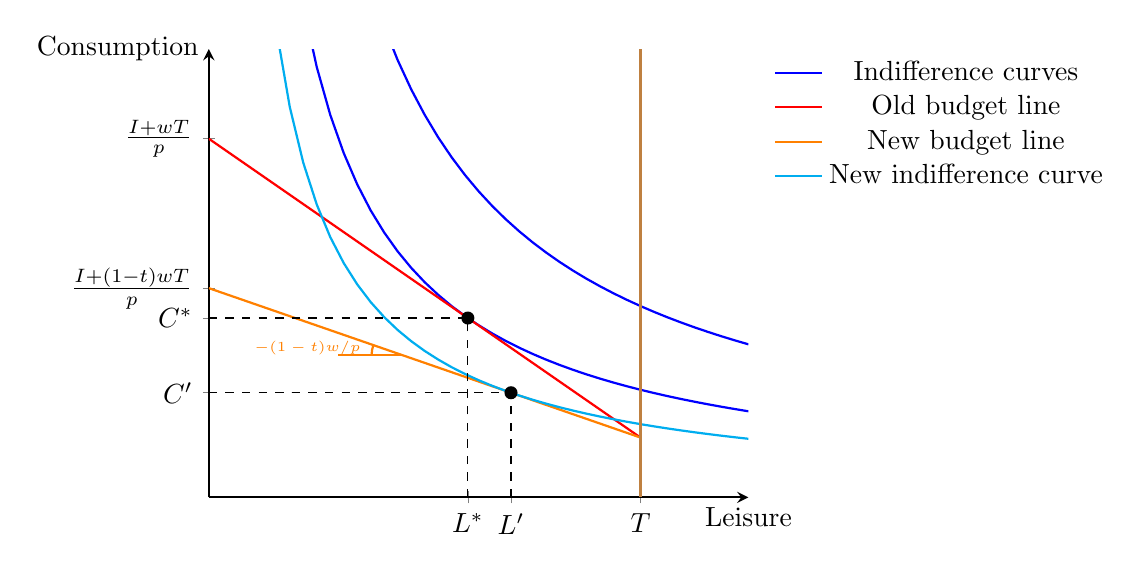
\begin{tikzpicture} 
\begin{axis}[%yticklabel style={/pgf/number format/fixed,},             
xlabel={Leisure}, 
ylabel={Consumption},
axis lines=middle,
samples = 41, 
% grid, 
thick,
domain = 0:25,
ymin = 0,
ymax = 30,
legend pos = outer north east,
legend style={draw=none},   % If we don't want borders around the legend
xlabel style={below},
ylabel style={left},
xtick = {0, 12, 14, 20},
xticklabels = {$0$, $L^*$, $L^\prime$, $T$},
ytick = {0, 7, 12, 14, 24},
yticklabels = {$0$, $C^\prime$, $C^*$, $\frac{I+(1-t)wT}{p}$, $\frac{I+wT}{p}$}
]
\addplot+[thick, mark = none, name path global = Indifference] { 12^2/x };
%\addlegendentry{Indifference curves}
% Old budget line
\addplot+[thick, mark = none, name path global = Budget, domain = 0:20] {24 - x};
%\addlegendentry{Old budget line}   %...
% New budget line   
\addplot+[orange, thick, mark = none, domain = 0:20] {4 + 0.5*20 - (1 - 0.5)*x};
%\addlegendentry{New budget line}   %...
% Another indifference curve
\addplot[thick, mark = none, blue] { 16^2/x };
% New indifference curve
\addplot[thick, mark = none, cyan] { ((14*7)^0.5)^2/x };
%\addlegendentry{New indifference curve}
% Vertical bar for the maximum amount of time
\addplot [thick, mark = none, name path global = new, brown] coordinates {(20, 0) (20, 30)}; 
%\addplot[dashed, domain = 0:20 , black, thin] {4};   % Consumption if leisure equals T: I/p 

% Old optimal bundle
\node[circle, scale = 0.5, fill = black] at (axis cs:12, 12) {};    
% New optimal bundle
\node[circle, scale = 0.5, fill = black] at (axis cs:14, 7) {};  
  
\addplot[dashed, black, thin] coordinates {(12, 0) (12, 12)};  % Optimal leisure decision 
\addplot[dashed, domain = 0:12 , black, thin] {12};   % Optimal consumption decision
\addplot[dashed, domain = 0:14 , black, thin] {7};   % new consumption decision
\addplot[dashed, black, thin] coordinates {(14, 0) (14, 7)};  % New leisure decision 

\legend{Indifference curves,
	Old budget line,
	New budget line,
	,
	New indifference curve,
	,
	,
	,
	,
}


% For the angle of the new budget line
\addplot[no marks, domain = 6:9, orange] {9.5};
\coordinate (A) at (8, 10);
\coordinate (B) at (9, 9.5);
\coordinate (C) at (8, 9.5);
\pic [draw=orange, -, angle radius=.4cm]{angle = A--B--C};
\node at (axis cs:7.5, 10) [orange, anchor=east] {\tiny $-(1-t)w/p$};

\end{axis}
\end{tikzpicture}	
\end{center}
\caption[Wage tax and labor supply decision]{Effect of a wage tax on labor supply decisions}
\end{figure}	
	
\section{International trade}
This section contains graphs of the impact of import tariffs and export subsidies.	

% Graph for surpluses with an import tariff
%\centering
\begin{figure}[H]
\begin{center}
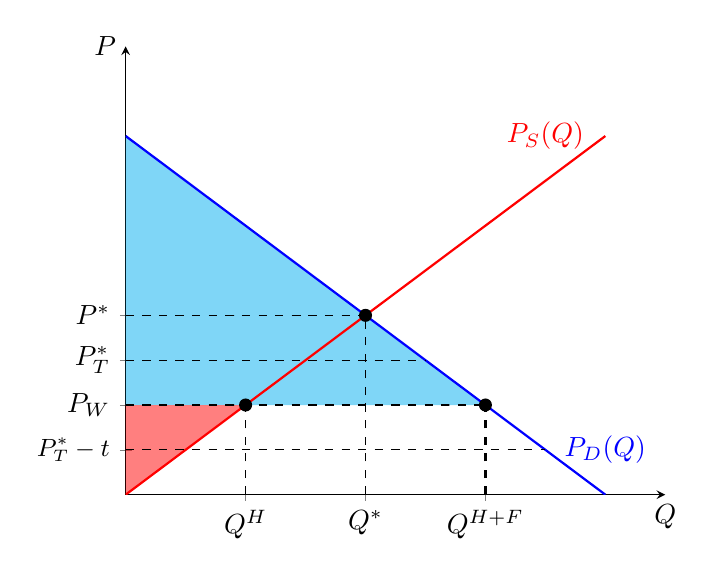
\begin{tikzpicture} 
\begin{axis}[
xlabel={$Q$}, 
ylabel={$P$},
axis lines= middle,
samples = 41, 
xmin = 0, xmax = 45,
ymin = 0, ymax = 100,
xtick = {0, 10, 20, 30} ,
xticklabels={$0$, $Q^H$, $Q^*$, $Q^{H+F}$},
ytick = {10, 20, 30, 40},
yticklabels={\small{$P_T^*-t$}, $P_W$, $P_T^*$, $P^*$ },
legend pos = outer north east,
legend style={draw=none},   % If we don't want borders around the legend
xlabel style={below},
ylabel style={left}]
% Inverse Demand
\addplot+[no marks, thick, name path = demand, domain = 0:40] {80- 2*x};
% Inverse Supply
\addplot+[no marks, thick, name path = supply, red, domain = 0:40] {2*x};
\addplot[ dashed, name path = pstar, domain = 0:20] {40};   % Old closed economy Equilibrium price
\addplot[ dashed, name path = pw, domain = 0:30, black ] {20};   % World price without a  tariff
\addplot[ dashed, name path = pt, domain = 0:25, black ] {30};   % World price after the tariff
\addplot[ dashed, name path = pt-t, domain = 0:35, black ] {10};   % pt - T 
\addplot[ dashed, black] coordinates {(20, 0) (20, 40)};  % Closed economy Equilibrium quantity
\addplot[ dashed, black] coordinates {(10, 0) (10, 20)};  % Open economy quantity produced by Home
\addplot[thick, dashed, black] coordinates {(30, 0) (30, 20)};  % Open economy quantity consumed in total
% Filling areas under the functions now
% Consumer surplus
\addplot [
thick,
color=cyan,
fill=cyan, 
fill opacity=0.5
]
fill between[
of=demand and pw,
soft clip={domain=0:30},
];

% Producer surplus
\addplot [
thick,
color=red,
fill=red, 
fill opacity=0.5
]
fill between[
of=pw and supply,
soft clip={domain=0:10},
];

% Government revenue
%\addplot[
%pattern = flexible hatch,
%yellow,
%fill=yellow, 
%fill opacity=0.5,
%postaction={pattern = north east lines, opacity = .5}
%]
%fill between[
%of=pprime-with-t and pprime,
%soft clip={domain=0:15},
%every segment no 1/.style={pattern = north west lines},
%];


% Deadweight loss
%\addplot [
%thick,
%color=green,
%fill=green, 
%fill opacity=0.5
%]
%fill between[
%of=demand and supply,
%soft clip={domain=15:20},
%];

%\legend{,
%	,
%	,
%	,
%	,
%	,
%	,
%	,
%	,
%	Consumer surplus,
%	Producer surplus
%}

\node[circle, scale = 0.5, fill = black] at (axis cs:20, 40) {};
\node[circle, scale = 0.5, fill = black] at (axis cs:10, 20) {};
\node[circle, scale = 0.5, fill = black] at (axis cs:30, 20) {};

% Label the demands and supply
\node[blue] at (axis cs: 40, 10) {$P_D(Q)$};
\node[red] at (axis cs: 35, 80) {$P_S(Q)$};

\end{axis}

\end{tikzpicture}
\end{center}
\caption[Surpluses after an import tariff]{Consumer and producer surpluses after an import tariff in a large economy}
\end{figure}

% Graph for surpluses with an import tariff
\begin{figure}[H]
\begin{center}
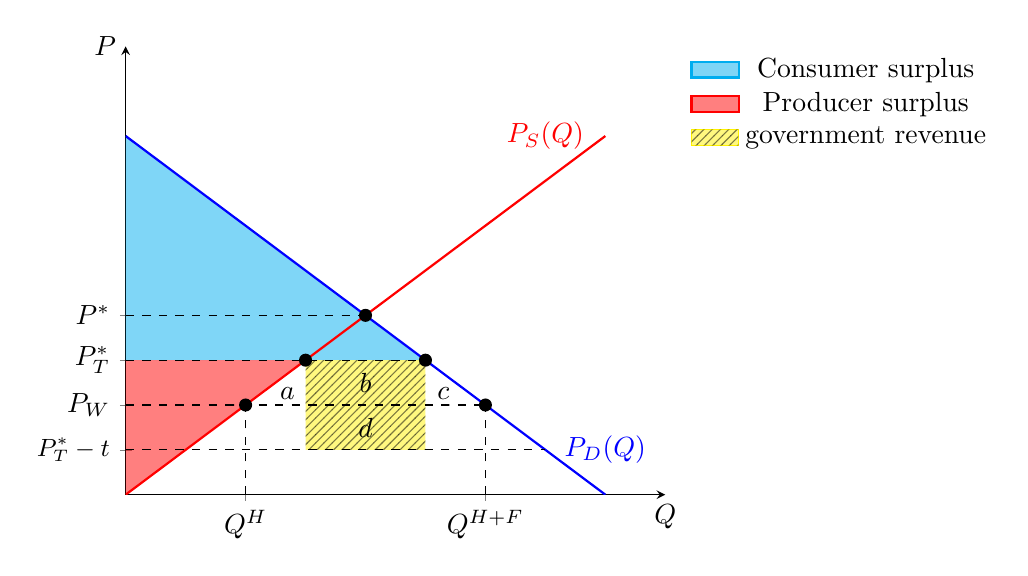
\begin{tikzpicture} 
\begin{axis}[
xlabel={$Q$}, 
ylabel={$P$},
axis lines= middle,
samples = 41, 
xmin = 0, xmax = 45,
ymin = 0, ymax = 100,
xtick = {0, 10, 30} ,
xticklabels={$0$, $Q^H$, $Q^{H+F}$},
ytick = {10, 20, 30, 40},
yticklabels={\small{$P_T^*-t$}, $P_W$, $P_T^*$, $P^*$ },
legend pos = outer north east,
legend style={draw=none},   % If we don't want borders around the legend
xlabel style={below},
ylabel style={left}]
% Inverse Demand
\addplot+[no marks, thick, name path = demand, domain = 0:40] {80- 2*x};
% Inverse Supply
\addplot+[no marks, thick, name path = supply, red, domain = 0:40] {2*x};
\addplot[ dashed, name path = pstar, domain = 0:20] {40};   % Old closed economy Equilibrium price
\addplot[ dashed, name path = pw, domain = 0:30, black ] {20};   % World price without a  tariff
\addplot[ dashed, name path = pt, domain = 0:25, black ] {30};   % World price after the tariff
\addplot[ dashed, name path = pt-t, domain = 0:35, black ] {10};   % pt - T 
%\addplot[ dashed, black] coordinates {(20, 0) (20, 40)};  % Closed economy Equilibrium quantity
\addplot[ dashed, black] coordinates {(10, 0) (10, 20)};  % Open economy quantity produced by Home
\addplot[ dashed, black] coordinates {(30, 0) (30, 20)};  % Open economy quantity consumed in total
% Filling areas under the functions now
% Consumer surplus
\addplot [
thick,
color=cyan,
fill=cyan, 
fill opacity=0.5
]
fill between[
of=demand and pt,
soft clip={domain=0:25},
];

% Producer surplus
\addplot [
thick,
color=red,
fill=red, 
fill opacity=0.5
]
fill between[
of=pt and supply,
soft clip={domain=0:15},
];

% Government revenue
\addplot[
%pattern = flexible hatch,
yellow,
fill=yellow, 
fill opacity=0.5,
postaction={pattern = north east lines, opacity = .5}
]
fill between[
of=pt and pt-t,
soft clip={domain=15:25},
every segment no 1/.style={pattern = north west lines},
];


% Deadweight loss
%\addplot [
%thick,
%color=green,
%fill=green, 
%fill opacity=0.5
%]
%fill between[
%of=demand and supply,
%soft clip={domain=15:20},
%];

\legend{,
	,
	,
	,
	,
	,
	,
	,
	Consumer surplus,
	Producer surplus,
	government revenue
}

\node[circle, scale = 0.5, fill = black] at (axis cs:10, 20) {};
\node[circle, scale = 0.5, fill = black] at (axis cs:15, 30) {};
\node[circle, scale = 0.5, fill = black] at (axis cs:20, 40) {};
\node[circle, scale = 0.5, fill = black] at (axis cs:25, 30) {};
\node[circle, scale = 0.5, fill = black] at (axis cs:30, 20) {};

% Label the demands and supply
\node[blue] at (axis cs: 40, 10) {$P_D(Q)$};
\node[red] at (axis cs: 35, 80) {$P_S(Q)$};
% locate the important areas
\node[black] at (axis cs: 13.5, 22.5) {$a$};
\node[black] at (axis cs: 20, 25) {$b$};
\node[black] at (axis cs: 26.5, 22.5) {$c$};
\node[black] at (axis cs: 20, 15) {$d$};

\end{axis}

\end{tikzpicture}
\end{center}
\caption[Import tariff in a large economy]{The impact of an import tariff in a large economy}
\end{figure}

% Graph for surpluses with an import tariff
\begin{figure}[H]
\begin{center}
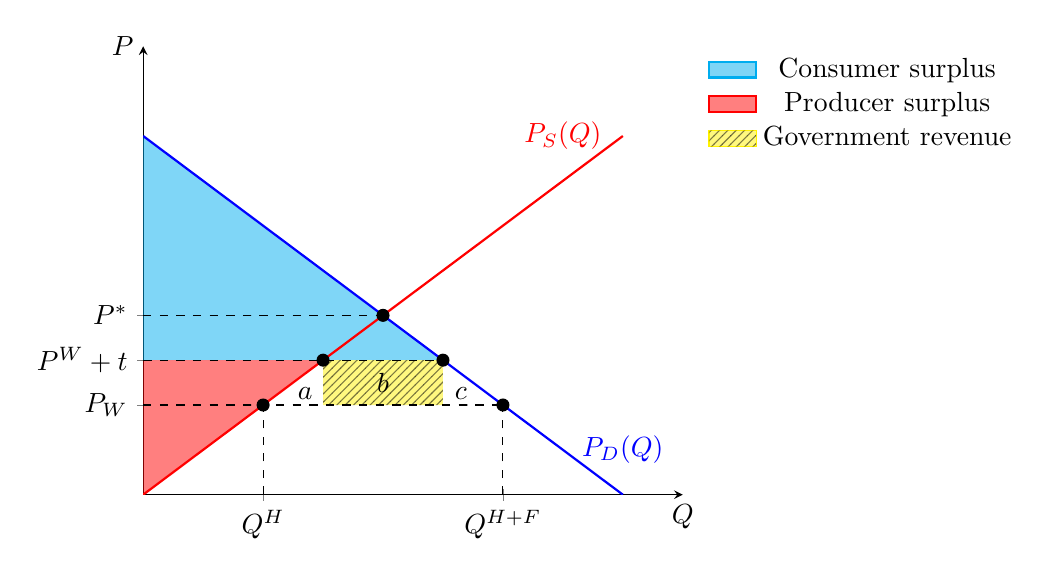
\begin{tikzpicture} 
\begin{axis}[
xlabel={$Q$}, 
ylabel={$P$},
axis lines= middle,
samples = 41, 
xmin = 0, xmax = 45,
ymin = 0, ymax = 100,
xtick = {0, 10, 30} ,
xticklabels={$0$, $Q^H$, $Q^{H+F}$},
ytick = {20, 30, 40},
yticklabels={ $P_W$, $P^W + t$, $P^*$ },
legend pos = outer north east,
legend style={draw=none},   % If we don't want borders around the legend
xlabel style={below},
ylabel style={left}]
% Inverse Demand
\addplot+[no marks, thick, name path = demand, domain = 0:40] {80- 2*x};
% Inverse Supply
\addplot+[no marks, thick, name path = supply, red, domain = 0:40] {2*x};
\addplot[ dashed, name path = pstar, domain = 0:20] {40};   % Old closed economy Equilibrium price
\addplot[ dashed, name path = pw, domain = 0:30, black ] {20};   % World price without a  tariff
\addplot[ dashed, name path = pt, domain = 0:25, black ] {30};   % World price after the tariff
%\addplot[ dashed, black] coordinates {(20, 0) (20, 40)};  % Closed economy Equilibrium quantity
\addplot[ dashed, black] coordinates {(10, 0) (10, 20)};  % Open economy quantity produced by Home
\addplot[ dashed, black] coordinates {(30, 0) (30, 20)};  % Open economy quantity consumed in total
% Filling areas under the functions now
% Consumer surplus
\addplot [
thick,
color=cyan,
fill=cyan, 
fill opacity=0.5
]
fill between[
of=demand and pt,
soft clip={domain=0:25},
];

% Producer surplus
\addplot [
thick,
color=red,
fill=red, 
fill opacity=0.5
]
fill between[
of=pt and supply,
soft clip={domain=0:15},
];

% Government revenue
\addplot[
%pattern = flexible hatch,
yellow,
fill=yellow, 
fill opacity=0.5,
postaction={pattern = north east lines, opacity = .5}
]
fill between[
of=pt and pw,
soft clip={domain=15:25},
every segment no 1/.style={pattern = north west lines},
];


% Deadweight loss
%\addplot [
%thick,
%color=green,
%fill=green, 
%fill opacity=0.5
%]
%fill between[
%of=demand and supply,
%soft clip={domain=15:20},
%];

\legend{,
	,
	,
	,
	,
	,
	,
	Consumer surplus,
	Producer surplus,
	Government revenue
}

\node[circle, scale = 0.5, fill = black] at (axis cs:10, 20) {};
\node[circle, scale = 0.5, fill = black] at (axis cs:15, 30) {};
\node[circle, scale = 0.5, fill = black] at (axis cs:20, 40) {};
\node[circle, scale = 0.5, fill = black] at (axis cs:25, 30) {};
\node[circle, scale = 0.5, fill = black] at (axis cs:30, 20) {};

% Label the demands and supply
\node[blue] at (axis cs: 40, 10) {$P_D(Q)$};
\node[red] at (axis cs: 35, 80) {$P_S(Q)$};
% locate the important areas
\node[black] at (axis cs: 13.5, 22.5) {$a$};
\node[black] at (axis cs: 20, 25) {$b$};
\node[black] at (axis cs: 26.5, 22.5) {$c$};
%\node[black] at (axis cs: 20, 15) {$d$};

\end{axis}

\end{tikzpicture}
\caption[Import tariff - small economy]{Surpluses after an import tariff in a small economy}
\end{center}	
\end{figure}

\section{Insurance}
In this section is exposed the optimal insurance decision of a risk averse agent facing a probability $1-\alpha$ of incurring a loss $L$ and a probability $\alpha$ of not incurring any loss. The agent's utility is concave, and the insurance policy rates are actuarially fair (the coverage per dollar $\pi$ equals $1-\alpha$, the probability of the loss occurring). Therefore, full insurance is optimal (point B) as opposed to no insurance (point A).


% Complete this section with the math details
\begin{figure}[H]
\begin{center}
\begin{tikzpicture} 
\begin{axis}[
xlabel={income in good state}, 
ylabel={income in bad state},
axis lines= middle,
%axis lines = left,
samples = 100,   % number of points used to draw the curves
xmin = 0, xmax = 5,  % boundaries on the axes
ymin = 0, ymax = 5,
xtick = {2.62, 1.5},  % Marks at some coordinates along the x-axis
xticklabels={$y$, $y^*$},  % Labels corresponding to the marks
ytick = {0.38, 1.5},  % Marks at some coordinates along the y-axis
%thick,   % Makes any curve thick. Can be individually included in each curve otherwise
yticklabels={ $y-L$, $y^*$ }, % Labels corresponding to the marks
%legend pos = outer north east,
legend style={draw=none, at = {(1.1, 1)}, font = \scriptsize},   % customize the legend: position, font size, box around the text
xlabel style={below}, % Place of the axes labels
ylabel style={left} ]

% An indifference curve (name path can be useful to refer to that curve later, like in the legend)
\addplot[thick, DarkRed, name path = indifference curve, domain = 0:5] {1/x};   
% Optimal indifference curve
\addplot[thick, DarkRed, name path = indifference curve, domain = 0:5] {(1.5)^2/x};   


% Budget line
\addplot[thick, darkcyan, name path = budget, domain = 0:5] {3-x};   
% Budget and indifference curve cross at 2.62 (solve 1/x = 3-x)
\addplot[dashed, black] coordinates {(2.62, 0) (2.62, 0.38)};  
\addplot[dashed, domain = 0:2.62] {0.38};   
\node[circle, scale = 0.5, fill = black] at (axis cs:2.62, 0.38 ) {};
% 45 degrees line
\addplot[dashed, domain = 0:3.7] {x};   
\node[black] at (axis cs: 3.9, 4) {$45^{\circ}$ line ($y_G=y_B$)};

% Full insurance point
\addplot[dashed, black] coordinates {(1.5, 0) (1.5, 1.5)};  
\addplot[dashed, domain = 0:1.5] {1.5}; 
\node[circle, scale = 0.5, fill = black] at (axis cs:1.5, 1.5 ) {};  

% Arrows describing slopes
\draw[->, thick, darkcyan] (axis cs:1.5, 3.9) -- (axis cs:0.8, 2.3);
\draw[->, thick, DarkRed] (axis cs:3.9, 1.2) -- (axis cs:3.9, 0.3);
%\draw[->, thick] (axis cs:0.55, 0.55) -- (axis cs:0.7, 0.7);
\node[darkcyan] at (axis cs: 1.5, 4) {slope = $-\frac{\alpha}{1-\alpha}$};
\node[DarkRed] at (axis cs: 3.9, 1.5) {slope = -$\frac{\alpha u^\prime(y_G)}{(1-\alpha)u^\prime(y_B)}$};

% Label points A and B
\node[black] at (axis cs: 1.5, 1.8) {B};
\node[black] at (axis cs: 2.8, 0.6) {A};

\end{axis}

\end{tikzpicture}
\end{center}
\caption[Optimal insurance decision]{Optimal insurance decision}
\end{figure}	

\section{Game theory}
This section contains graphs for Nash equilibria in simultaneous moves games, as well as normal and extensive form games. 
The first graph shows the Nash equilibrium in mixed strategies in the ``matching pennies'' game.
% Graph for the matching pennies game best response and Nash equilibrium
\begin{figure}[H]
\begin{center}
\begin{tikzpicture} 
\begin{axis}[
xlabel={$q$}, 
ylabel={$p$},
axis lines= middle,
%axis lines = left,
samples = 41, 
xmin = -0.1, xmax = 1.2,
ymin = -0.1, ymax = 1.2,
xtick = {0, 1/2, 1} ,
xticklabels={$0$, $1/2$,  $1$},
ytick = {1/2, 1},
%thick,
yticklabels={ $1/2$, $1$ },
%legend pos = outer north east,
legend style={draw=none, at = {(1.1, 1)}, font = \scriptsize},   % customize the legend: position, font size, box around the text
xlabel style={below},
ylabel style={left}]

% Best response functions. 
% Row's choice of q
\addplot[thick, darkcyan, name path = Row's BR] coordinates {(0, 0) (0, 1/2)}; 
\addplot[thick, darkcyan, domain = 0:1] {1/2};   % 
\addplot[thick, darkcyan] coordinates {(1, 1/2) (1, 1)}; 

% Column's choice of p
\addplot[thick, DarkRed, name path = Column's BR , domain = 0:(1/2)] {1};   % 
\addplot[thick, DarkRed] coordinates {(1/2, 0) (1/2, 1)}; 
\addplot[thick, DarkRed, domain = (1/2):1] {0};   % 

\node[circle, scale = 0.5, fill = black] at (axis cs:1/2, 1/2) {};

\node[black] at (axis cs: -0.05, -0.05) {$0$};

\legend{Row's BR $q(p)$,
	,
	,
	Column's BR $p(q)$
}

\node[black] at (axis cs: 0.3, 0.7) {\textbf{NE}};
% NE arrows
\draw[->, thick] (axis cs:0.35, 0.65) -- (axis cs:0.45, 0.55);
%\draw[->, thick] (axis cs:0.55, 0.45) -- (axis cs:0.95, 0.05);
%\draw[->, thick] (axis cs:0.55, 0.55) -- (axis cs:0.7, 0.7);
\end{axis}
\end{tikzpicture}	
\caption[Mixed strategies NE - Chicken game]{Mixed strategies Nash equilibrium in the Chicken game}
\end{center}
\end{figure}


The next graph shows the Nash equilibria in a ``chicken game''. There are 2 Nash equilibria in pure strategies, and 1 in mixed strategies.	
% Graph for the Nash equilibria in a chicken game
\begin{figure}[H]
\begin{center}
\begin{tikzpicture} 
\begin{axis}[
xlabel={$q$}, 
ylabel={$p$},
axis lines= middle,
%axis lines = left,
samples = 41, 
xmin = -0.1, xmax = 1.2,
ymin = -0.1, ymax = 1.2,
xtick = {0, 3/4, 1} ,
xticklabels={$0$, $3/4$,  $1$},
ytick = {3/4, 1},
%thick,
yticklabels={ $3/4$, $1$ },
%legend pos = outer north east,
legend style={draw=none, at = {(1.1, 1)}, font = \scriptsize},   % customize the legend: position, font size, box around the text
xlabel style={below},
ylabel style={left}]

% Best response functions. Separate lines right now, see if I can make kink functions later
\addplot[thick, DarkRed, name path = James' BR , domain = 0:(3/4)] {1};   % 
\addplot[thick, DarkRed] coordinates {(0.75, 0) (0.75, 1)}; 
\addplot[thick, DarkRed, domain = (3/4):1] {0};   % 


\addplot[thick, darkcyan, name path = Dean's BR] coordinates {(0, 0.75) (0, 1)}; 
\addplot[thick, darkcyan, domain = 0:1] {3/4};   % 
\addplot[thick, darkcyan] coordinates {(1, 0) (1, 3/4)}; 

\node[circle, scale = 0.5, fill = black] at (axis cs:1, 0) {};
\node[circle, scale = 0.5, fill = black] at (axis cs:0, 1) {};
\node[circle, scale = 0.5, fill = black] at (axis cs:3/4, 3/4) {};

\node[black] at (axis cs: -0.05, -0.05) {$0$};



\legend{Dean's BR $p(q)$,
	,
	,
	James' BR $q(p)$,
}

\node[black] at (axis cs: 0.5, 0.5) {\textbf{NE}};
% NE arrows
\draw[->, thick] (axis cs:0.45, 0.55) -- (axis cs:0.05, 0.95);
\draw[->, thick] (axis cs:0.55, 0.45) -- (axis cs:0.95, 0.05);
\draw[->, thick] (axis cs:0.55, 0.55) -- (axis cs:0.7, 0.7);

\end{axis}
\end{tikzpicture}	
\end{center}
\caption[Nash equilibria in the chicken game]{Nash equilibria in the chicken game}
\end{figure}

Consider the following simultaneous moves game:
\begin{center}
\begin{game}{2}{2}[\textbf{\color{darkcyan} Girl}][\textbf{\color{DarkRed} Sanji}][\textbf{\color{darkolivegreen} Avoiding Sanji}]       \> Party 1   \> Party 2\\ Party 1  \>$5,15$   \>$20,10$\\ Party 2    \>$15,5$   \>$0,20$ 
\end{game} 
\end{center}

The following tree shows a version of the game played sequentially. Here the girl gets to make the first move:
\begin{figure}[H]
\begin{center}
\begin{tikzpicture}[scale=1.3,font=\footnotesize, edge from parent/.style={draw,thick}]
			% Two node styles for game trees: solid and hollow
			
			\tikzstyle{solid node}=[circle,draw,inner sep=1.5,fill=black];
			\tikzstyle{hollow node}=[circle,draw,inner sep=1.5];
			\tikzstyle{level 1}=[level distance=15mm,sibling distance=3.5cm]
			\tikzstyle{level 2}=[level distance=15mm,sibling distance=1.5cm]
			
			% The tree
			\node(0)[hollow node,label=above:{\color{darkcyan}$Girl$}]{}
			child{node[solid node,label=above left:{\color{DarkRed}$Sanji$}]{}
				child{node(gna)[label=below:{$\left(\begin{array}{c} 20\\ 10 \end{array}\right)$}]{} edge from parent [black] node[left]{P2}}
				child{node[label=below:{$\left(\begin{array}{c} 5\\ 15 \end{array}\right)$}]{} edge from parent [red] node[right]{P1}}
				edge from parent [red] node[left,xshift=-5]{P1}
			}
			child{node[solid node,label=above right:{\color{DarkRed}$Sanji$}]{}
				child{node[label=below:{$\left(\begin{array}{c} 0\\ 20 \end{array}\right)$}]{} edge from parent [red] node[left]{P2}}
				child{node[label=below:{$\left(\begin{array}{c} 15\\ 5 \end{array}\right)$}]{} edge from parent node[right]{P1}}
				edge from parent node[right,xshift=5]{P2}
			};
			
			\draw[draw=white](gna)--+(-.9,-.5)node[left]
			{$\left(\begin{array}{c} {\color{darkcyan}Girl}\\ {\color{DarkRed}Sanji} \end{array}\right)$};
		\end{tikzpicture}
\end{center}
\caption[A sequential game tree]{A sequential game tree}
\end{figure}	
		
The notorious centipede game is in the following tree:
\begin{figure}[H]
\begin{center}
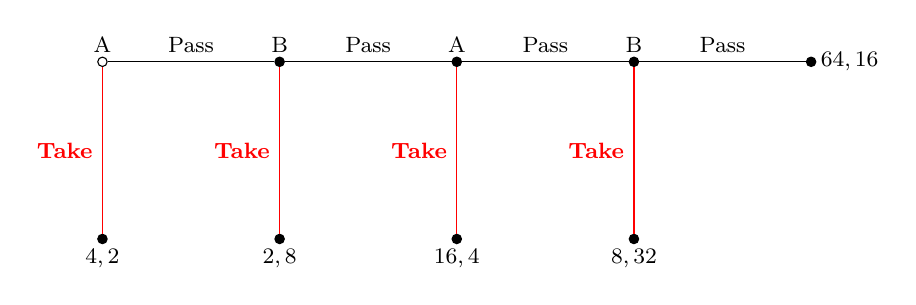
\begin{tikzpicture}[font=\footnotesize,scale=1.5]
% Two node styles: solid and hollow
\tikzstyle{solid node}=[circle,draw,inner sep=1.2,fill=black];
\tikzstyle{hollow node}=[circle,draw,inner sep=1.2];
% The Tree
\node(0)[hollow node]{}
child[grow=down]{node[solid node]{}edge from parent[red] node[left]{\textbf{Take}}}
child[grow=right]{node(1)[solid node]{}
child[grow=down]{node[solid node]{}edge from parent[red] node[left]{\textbf{Take}}}
child[grow=right]{node(2)[solid node]{}
child[grow=down]{node[solid node]{}edge from parent[red] node[left]{\textbf{Take}}}
child[grow=right]{node(3)[solid node]{}
child[grow=down]{node[solid node]{}edge from parent[red] node[left]{\textbf{Take}}}
child[grow=right]{node(4)[solid node]{}edge from parent node[above]{Pass}}edge from parent node[above]{Pass}}edge from parent node[above]{Pass}}edge from parent node[above]{Pass}};
%child[grow=down]{node[solid node]{}edge from parent node[left]{$S$}}
%child[grow=right]{node(5)[solid node]{}%child[grow=down]{node[solid node]{}edge from parent node[left]{$S$}}
%child[grow=right]{node(6)[solid node]{}
% Movers

\foreach \x in {0,2}
\node[above]at(\x){A};
\foreach \x in {1,3}
\node[above]at(\x){B};
% payoffs
\node[below]at(0-1){$4,2$};
\node[below]at(1-1){$2,8$};
\node[below]at(2-1){$16,4$};
\node[below]at(3-1){$8,32$};

\node[right]at(4){$64,16$};
\end{tikzpicture}
\end{center}
\caption[The centipede game]{The centipede game}
\end{figure}

\section{Program evaluation methods}

Program evaluation methods aim at estimating the causal impact of some intervention (or treatment) labelled $D_i$ on some outcome variable $Y_i$. Depending on the design of the intervention, different methods will be employed. For 2 methods in particular, a graphic illustration helps understand the mechanics of the method. 

\subsection{Difference-in-differences (Did)}
When randomized control trials are not feasible, natural experiment can be used to estimate the average treatment effect on the treated (ATT). Because Selection into the treatment is not random in a natural experiment, one can rely on the comparison in the time variation for treatment and control group. Under the \textbf{parallel tends assumption} (in the absence of treatment, the control and treatment groups would have evolved the same way over time), the difference in the time variation delivers a consistent estimate of the ATT. It can be estimated via the following equation:
\[
Y_{i,t} = \beta_0 + \tau D_i + \lambda D_t + \delta \left(D_i\times D_t  \right) + X_{i,t}^{\prime}\beta_1 + \varepsilon_{i,t}
\]
where $D_t$ is a dummy variable equal to 1 if observation $i$ occurs after the treatment, and equal to 0 if it occurs before, $D_i$ is the treatment dummy variable, and $X_{i,t}$ is a set of additional covariates. The ATT is given by $\delta$, and all the coefficients can be represented in the following graph (the treatment group is represented in {\color{darckcyan}blue}, the treatment group in {\color{DarkRed}red}): 

\begin{figure}[H]
\begin{center}
\begin{tikzpicture} 
\begin{axis}[
xlabel={Time}, 
ylabel={$Y$},
axis lines= middle,
samples = 41, 
xmin = 10, xmax = 110,
ymin = 0, ymax = 100,
tick style={draw=none},
xtick = {0, 15, 50, 85} ,
xticklabels={$0$, before, treatment, after},
ytick = { },
yticklabels={ },
legend pos = outer north east,
legend style={draw=none},   % If we don't want borders around the legend
xlabel style={below},
ylabel style={left}]

% Time of the treatment
\addplot[black] coordinates {(50, 0) (50, 90)}; 
\addplot[dashed, black] coordinates {(15, 0) (15, 100)}; % Before the treatment
\addplot[dashed, black] coordinates {(85, 0) (85, 100)}; % After the treatment
% Control group
\addplot[DarkRed, thick, mark=*] coordinates {(15, 15) (85, 35)};
\addplot[DarkRed, thick, dashed, mark=*] coordinates {(15, 15) (85, 15)};
%\draw [black, thick] [<->](25, 30)--(75, 50) ;  
% Treatment group
\addplot[darkcyan, thick, mark=*] coordinates {(15, 40) (85, 90)};
\addplot[gray, thick, dashed, mark=*] coordinates {(15, 40) (85, 60)};
\addplot[darkcyan, thick, dashed, mark=*] coordinates {(15, 40) (85, 40)};
%\draw [black, thick] [<->](25, 50)--(75, 70) ;

% Curly brackets to describe ATT = delta + lambda
\draw [darkcyan, thick, decorate, decoration={brace, raise = 5pt, amplitude = 5pt, mirror}]
(85, 40) -- (85, 90)node [black, midway, right=10pt] {\scriptsize{${\color{darkcyan}ATT} + {\color{SFUgold}a}$}};

% Curly brackets to describe the differences between groups
%\draw [orange, thick, decorate, decoration={brace, raise = 5pt, amplitude = 5pt, mirror}]
%(15, 15) -- (15, 40)node [orange, midway, right=10pt] {\footnotesize{$\tau$}};

% Curly brackets to describe the intercept
%\draw [darkolivegreen, thick, decorate, decoration={brace, raise = 5pt, amplitude = 5pt, mirror}]
%(15, 0) -- (15, 15)node [darkolivegreen, midway, right=10pt] {\footnotesize{$\beta_0$}};

% Curly brackets to describe the time fixed effect
\draw [SFUgold, thick, decorate, decoration={brace, raise = 5pt, amplitude = 5pt, mirror}]
(85, 15) -- (85, 35)node [SFUgold, midway, right=10pt] {\footnotesize{$a$}};

%\node[circle, scale = 0.5, fill = black] at (axis cs:70, 35) {};
%\node[circle, scale = 0.5, fill = black] at (axis cs:52.5, 52.5) {};

\end{axis}

\end{tikzpicture}
\end{center}
\caption{Difference-in-differences estimation decomposition}
\end{figure}

Note the presence of curly brackets using the command
\begin{lstlisting} 
\draw [darkcyan, thick, decorate, decoration={brace, raise = 5pt, amplitude = 5pt, mirror}]
(85, 40) -- (85, 90)node [black, midway, right=10pt]
\end{lstlisting} 

\subsection{Regression Discontinuity Designs (RDD)}	
There are instances where the assignment to treatment is a deterministic function of some variable. Crossing such a threshold can define a discontinuity in the outcome variable, and under the \textbf{continuity assumption}, the cause of that jump is due to the treatment only. Observations on either side of the threshold can be considered comparable, if not for their treatment status. Hence, such designs help estimate a \textbf{Local Average Treatment Effect (LATE)}. The design is explained best with a graph around the cutoff point:

\pgfplotstableread{RDD.dat}{\table}  % loads data to be plotted

\begin{figure}[H]
\begin{center}
\begin{tikzpicture} 
\begin{axis}[
xlabel={$X$}, 
ylabel={$Y$},
axis lines= middle,
samples = 41, 
xmin = 47, xmax = 53,
ymin = 40, ymax = 70,
tick style={draw=none},
xtick = {0, 50} ,
xticklabels={$0$, $c$},
ytick = { },
yticklabels={ },
legend pos = outer north east,
legend style={draw=none},   % If we don't want borders around the legend
xlabel style={below},
ylabel style={left}]

 % Cutoff point
\addplot[black, dashed] coordinates {(50, 40) (50, 70)}; 
% Scatter plot of the data (generated in R)
\addplot[orange, only marks, , mark size = 1pt] table [x = {x}, y = {y}] {\table};

\end{axis}

\end{tikzpicture}
\end{center}
\caption[RDD]{Regression Discontinuity Design}
\end{figure}

This graph was produced using data generated in \textbf{\textsf{Rstudio}}, converted into the .dat format (other statistical software such as Matlab or Stata can also be used for that purpose). The data were loaded in Latex using \begin{lstlisting} 
\pgfplotstableread{RDD.dat}{\table} 
\end{lstlisting} 
The data will automatically appear in the graph, what is left to do is design the format of the graph itself (axes range, cutoff point, lables, etc)
	
\end{document}
